% LaTeX thesis template.
% Version 1.6
%
% Department of Computer Science IV,
% University of Mannheim,
% Germany
%
% Based on the KOMA script classes.
% Created by Philip Mildner 2013-2015.
% If you have any feedback or if you find errors contact me:
% mildner@informatik.uni-mannheim.de
%
% Relevant class options:
%
% oneside:
% For shorter thesis like seminar papers you can use the single-sided layout, for longer thesis
% the double-sided layout is preferred (and it uses less paper, too). If you would like to have
% a single-sided print, use the 'oneside' option in the documentclass.
%
% BCOR=<value>:
% Depending on your method of binding, you might want to change the BCOR setting to account for
% the part of the pages that are hidden in the cover (e.g., set 'BCOR=10mm' if 1cm is hidden). 
%
% german:
% The standard behavior of this template is to produce English documents. If you would like to
% write your work in German, just include the 'german' option.
%
% draft:
% If you set the 'draft' option, overfull boxes will be highlighted in the PDF file so that you can
% find them more easily.

\documentclass[twoside,BCOR=12mm]{pi4-thesis}

% additional packages
\usepackage{tikz}
\usetikzlibrary{shapes,arrows,positioning}
\usepackage{tikz-uml}
\usepackage[linesnumbered,ruled,vlined]{algorithm2e}
\usepackage{pgfplots}
\usepackage{colortbl}
\usepackage{lscape}
\usepackage{theorem}

% additional styles
\tikzstyle{line} = [draw, -latex']
\theoremstyle{break}
\setlength\theorempreskipamount{3ex}
\setlength\theorempostskipamount{3ex}
\newtheorem{define}{Definition}
\newtheorem{hypothesis}{Hypothesis}

% The title page in this template has a pretty standard layout. While all relevant information are
% displayed on it, it surely could be improved to look nicer. You are invited to change the title
% page to your needs. If you have found a pleasing layout, I will be glad if you share it with me.
%
% Fill in the relevant information in the following lines.
%
% Choose between bachelor thesis or master thesis.
\piivsubject{Master Thesis}
% The title of your work.
\piivtitle{Comparison of Disparity Algorithms for Stereoscopic Video}
% Your name.
\piivauthor{Ben John}
% Name of your supervisor.
\piivsupervisor{Dr. Stephan Kopf}
% The date you submit your thesis. You can substitute the command with any date.
\date{May 2016}

% If you want to use the glossary make sure your 'makeindex' toolchain is working correctly.
% Alternetively, you might want to look into the 'xindy' option of the glossaries package.
\makeglossaries

\begin{document}

% -----------------------------------------------------------------------------
% Acronyms Begin
\newacronym{hdr}{HDR}{High Dynamic Range}

\newacronym{ctan}{CTAN}{The Comprehensive \TeX{} Archive Network}

\newacronym{fim}{FIM}{Fachschaft für Mathematik und Informatik}
% Acronyms End
% -----------------------------------------------------------------------------
% -----------------------------------------------------------------------------
% Main Glossary Begin
\newglossaryentry{seam_carving}
 {
   name=Seam Carving,
   description={Seam carving describes an algorithm to rescale images. Originally proposed by Avidan and Shamir, it has been further developed and adapted for videos. Instead of just cropping or rescaling an image, single seams through the image are identified that are least significant to the image's content}
}
% Main Glossary End
% -----------------------------------------------------------------------------

% Abstract is optional. If you do not use an abstract, remove it.
% ---------------------------------
% Begin of abstract
\abstractchap
Stereoskopische Videos speichern zwei separate Ansichten einer Szene, die sich {\"u}blicherweise nur in geringen horizontalen Verschiebungen der Pixel unterscheiden. Diese Pixelverschiebungen (Disparity) resultieren aus den unterschiedlichen Entfernungen der Objekte in der Szene. Ziel der Master-Abschlussarbeit ist es, bestehende Verfahren zur Berechnung der Disparity zu analysieren, geeignete Verfahren f{\"u}r Videos auszuw{\"a}hlen und diese zu implementieren. Ein spezieller Fokus soll auf Erweiterungen f{\"u}r Videos liegen, indem beispielsweise vorherige oder zuk{\"u}nftige Frames ber{\"u}cksichtigt werden. Zur Messung der Qualit{\"a}t der implementierten Verfahren sollen bestehende stereoskopische Bild- und Videoarchive genutzt werden.

% End of abstract
% ---------------------------------

% ---------------------------------
% Begin of listings
\microtypesetup{protrusion=false} % disables protrusion locally in the document
\tableofcontents
% If you should not have any figures, tables or acronyms in your paper remove the according list.
\listoffigures
\listoftables

%\listofalgorithms
%\addcontentsline{toc}{chapter}{List of Algorithms}

% Uncomment the next line if you use listings in your document.
% \lstlistoflistings
\microtypesetup{protrusion=true} % enables protrusion

\printglossary[type=\acronymtype]
% End of listings
% ---------------------------------

% ---------------------------------
% Begin of main part
\mainmatter

\chapter{Introduction}
\label{chap:introduction}

\section{Motivation}

Computer vision establishes itself on the consumer market as more research is done.
The upcoming iPhone supports this as it will feature a dual camera system \footnote{\url{http://9to5mac.com/2016/02/03/sony-dual-cameras-iphone-7-plus/}, 2016-02-22.}.
In the year 2011 LG and HTC released the LG Optimus 3D\footnote{\url{https://en.wikipedia.org/wiki/LG_Optimus_3D} } and corresponding the HTC Evo 3D\footnote{\url{https://en.wikipedia.org/wiki/HTC_Evo_3D}}.
Both had a stereo camera implemented and an auto-stereoscopic display attached.
This enables one to view photos or videos taken in stereographic 3D without the actual need for additional peripheral like 3D glasses.
Both can be seen as an experiment as there was no big distribution, Apple normally focuses on the mainstream consumer market, opening up the box of possibilities and the need for such algorithms even further.
One example application for such a consumer-driven market could be the reconstruction of a face after taking a photo.
There exist no method to reconstruct a whole 3D model without having stereo images from all angles of the face, but it is possible to trick the user in having captured a 3D photo.
Another concrete example for an application regarding depth estimation in stereo videos is to detect moving people in a stereo video and calculate the distance to the camera of each person\footnote{\url{http://de.mathworks.com/help/vision/examples/depth-estimation-from-stereo-video.html}}.
\newline\newline\noindent Obtaining depth information as additional data to infer intents from human gestures has arrived in mainstream computing with the release of Kinect at November 4th, 2010.
Kinect is a hardware add-on for the Xbox video gaming console which enables users to interact visually with the console without actually using a controller or any other peripheral.
The Kinect for Xbox one utilizes two cameras, one capturing colored and the other monochrome images.
The monochrome sensor is used in combination with an infrared laser projector to obtain depth information via time of flight (TOF).
Time of flight is a method to measure the time light needs to reach objects and then to calculate the distance.
\newline\newline\noindent With deducing intents from human gestures a step in the field of artificial intelligence was made as the computer is now able to interpret human body language.
As this means processing an enormous stream of data (gathering and processing frame by frame) it represents a dataset of large and complex nature, also known as big data.
This also implies the need for new data processing techniques in comparison with traditional ones.
As a result one could say that computer vision is linked to both, artificial intelligence and big data.
New applications which arose from the combination of those topics are for instance:

\begin{itemize}
  \item robotic and autonomous driving,
  \item medical image analysis and automatic surgery,
  \item 3DTV and video compression.
\end{itemize}

\noindent Besides the technology of time of flight laser sensors - such as the Kinect\footnote{Besides the consumer market, for autonomous driving or robotic research Velodyne is a well-known sensor.} - there exists also the possibility to obtain depth information from stereo images by analyzing coherent images with so called disparity algorithms.
Thus, it is sufficient to have two calibrated aligned cameras (a stereo camera) to acquire disparity information and calculate the depth at each point.
But this leads to another fundamental problem of stereo matching: stereo correspondence.
Basically, stereo correspondence means the labelling of pixels, i.e. which pixel of the left image belongs to the corresponding pixel on the right image as a projection of the same three-dimensional point from the captured world, projected to the image plane in every image.
This problem of stereo correspondence has to be solved in order to actually match those and calculate the disparity.
According to \citeauthor{scharstein2002taxonomy}, stereo correspondence is one of the most heavily investigated topics in computer vision \citep{scharstein2002taxonomy}.
As there is still a lot of research going on, no algorithm is working without any mistakes and also the runtime is a bit quirky, Microsoft Kinect established itself as a real alternative.
This leads us to one of the disadvantages of Kinect sensor: Kinect is sensitive to other infrared sources (like sunlight) due to its nature of utilizing an infrared laser projector to acquire depth information, a stereo camera does not have this issue.
Although using two coherent images also have some disadvantages which will be discussed later on, it is an alternative way to receive depth information.
Especially thinking about autonomous driving during which at day a lot of sunlight is involved in, other techniques to estimate how far an object is away from one another are necessary to ensure a certain accuracy and fault-tolerance.

\section{Assignment}

The thesis' main goal is to provide an overview of selected disparity algorithms for stereoscopic videos and evaluate those.
\citeauthor{scharstein2002taxonomy} justified their tiny selection of disparity algorithms with the following: "Compiling a complete survey of existing stereo methods [...] would be a formidable task, as a large number of new methods are published every year." \citep{scharstein2002taxonomy}.
That said the ones with well documented source code and a research paper, also adaptable within the time scope of this thesis, were integrated.
The main assignments can be summarized in three research tasks:

\begin{itemize}
  \item Providing fundamental knowledge of existing stereo matching algorithms to have a basis for an advanced insight into the area of disparity algorithms targeting stereoscopic videos.
  \item Implementation of a stereo matcher for videos utilizing the OpenCV library. The implemented stereo matcher should be enhanced by using a spatiotemporal context
  \item Evaluation of the presented algorithms by implementation and presentation of an evaluation suite. Existing datasets, as well as a novel Dataset of the Department of Praktische Informatik IV\footnote{\url{http://ls.fmi.uni-mannheim.de/de/pi4/}} will thereby be examined using a set of defined quality metrics for assessment of the algorithms together with their runtime. Results are presented on a web-frontend.
\end{itemize}

\section{Outline}

The main purpose of Chapter \ref{chap:foundations} is to give an overview of terms and techniques used in this thesis.
The following Chapter \ref{chap:related} focuses more on disparity algorithms and related work.
To give an overview of state of the art algorithms a small summary of current used disparity algorithms is made.
This will create the foundations for the later implementation.
Chapter \ref{chap:impl} describes the implementation and explains reasons for building an evaluation engine.
The details of the implementation are explained afterwards.
In addition, the integration of existing algorithms is illustrated.
The evaluation engine was fed with datasets which are introduced in Chapter \ref{chap:eval}.
This chapter also explains the used quality metrics and describes the resulting outcome.
In the end, the results of this thesis are reflected in the concluding Chapter \ref{chap:conclusion}.
Besides some future work is pointed out.


\chapter{Foundations}
\label{chap:foundations}

In this chapter the foundations for related work and the implementation is built.
As a first step computer vision is introduced with a short explanation how image representation works from a computer's perspective.
Human visual perception is put in contrast to how computers perceive and interpret their environment.
In addition the labelling problem regarding stereo correspondence and the disparity between stereo images is illustrated.
Furthermore, the depth calculation as well as the taxonomy of disparity algorithms is depicted.
Finally, optical flow, a technical method that measures direction and movement of every pixel based on dominant movement in the original scene, is introduce to round this chapter up.

\section{Computer vision}

Computer graphics describes the terms and definitions of everything which has to do with basically treating images programmatically on a computer, interpreting and working with them.
To give an example, the applications of computer graphics range from image representation, image creation, image transformations to applications of color models.
Computer vision shares concepts from the domain of computer graphics, but works in reverse.
Instead of modeling a scene and generating an image of it, computer vision optically measures the real world and tries to analyze it by applying models to the captured images.
For instance trying to get information out of an image, like image segmentation, edge detection, classification and feature\footnote{Geometric shapes or more complex classifiers that are clearly recognizable.} points.
\newline\newline\noindent A simple example would be to imagine a face of a human being captured by a camera, which may produce errors due to lens distortion, shaky capturing and sampling of the chip.
Image editing would be useful to optimize the image by correction of contrast or brightness, cropping or further adjustments.
The tasks of computer vision are more in analyzing and understanding images for instance (just to name a few):

\begin{itemize}
  \item face detection to know the areas of faces on images,
  \item feature matching to detect the face on other images,
  \item feature tracking to track the movement of a person,
  \item 3D reconstruction of a facial model.
\end{itemize}

\subsection*{Image representation}

The existing method of handling images on a computer is separated into two different methods.
On the one hand a vector image describes its contents by representing forms like a circle, line, curve or rectangle.
The properties of these forms and shapes are also included, for instance coloring, size and origin.
So a vector image basically contains those forms and shapes, their properties and a description of how they are all composed together.
\newline\newline\noindent On the other hand as it may become pretty complex using vector images to represent the real-world, in contrast to those there also exist raster images.
Raster images (sometimes the term bitmap images is used) are a form to represent natural images, e.g. captured by a CCD\footnote{charge-coupled device} image sensor from a digicam.
Capturing means sampling information on a matrix of light sensitive sensors to transform received signals into color a matrix of the same size.

\begin{figure}[h!]
  \centering
  \includegraphics[width=0.5\textwidth]{src/images/rgb-raster-image.png}
  \caption[Example of a RGB raster image]{Example of a RGB raster image\protect\footnotemark}
  \label{fig:rgb-raster-image}
\end{figure}
\footnotetext{Source (accessed 02/2016): \url{https://en.wikipedia.org}.}

\noindent Both types of images use a coordinate system to describe either the placement of elements (like written above with the properties size and origin of each element) or to describe how each point looks like.
The coordinate system most widely used working with images starts in the upper left at the point $(0,0)$, with the x-axis extending to the right and y-axis extending to the bottom.
This can be seen as a grid system with the size of the image $width\ \times\ height$ representing $columns\ \times\ rows$.
By describing how each point looks like the exact description of a pixel is meant \citep{shirley2009fundamentals}.
\newline\newline\noindent One pixel in a grayscale image can range from $0 - 255$ describing the intensity of this pixel.
$0$ means black and $255$ is fully white.
In colored images a pixel can have more than one intensity value.
More concrete in a typical RGB\footnote{red-green-blue color channels} raster image each pixel contains three color channels, also called the RGB tuple.
Thus $$3 \cdot 1\ bytes = 3 \cdot 8\ bits = 3 \cdot 8 = 24\ bits$$ are saved per pixel utilizing RGB tuples.
In \texttt{C} or \texttt{C++} such pixel values are normally described as unsigned chars. A char represents one byte and unsigned means that it ranges from $0 - 255$ instead of $-128$ to $127$.
Sometimes RGB is used with an additional alpha channel specifying the degree of opacity, named RGBA\footnote{red-green-blue-alpha color channels}.
The composition of these color channels orchestrate the final pixel value as it is obtained by for example an image sensor.
Figure \ref{fig:rgb-raster-image} depicts an example of a RGB raster image and shows the values of three pixels.
The first marked pixel in figure \ref{fig:rgb-raster-image} describes the RGB tuple with the following values $(237,237,237)$.
Utilizing three color channels the final raster image then needs up to 24 bits per pixel, meaning an image the size $width = 300\ px$ and $height = 400\ px$ needs $$300 \cdot 400 \cdot 24bits \cdot \frac{1\ byte}{8\ bits} = 360.000\ bytes$$ in memory.
Images can be compressed with for example the JPEG algorithm but as the later implementation works only with pure raster images, as the unaltered values are examined, the amount of bytes as explained above is to be held in memory during the execution of the implementation.

\subsection*{Human visual perception}

In his manuscript 'Astronomia Pars Optica' from 1604, Kepler explains the use of both eyes for depth perception.
He defined the term binocular as the composition of two latin words, 'bini' for double and 'oculus' for eye.
With uniocular as 'uni' for one the sight with only one eye is meant.
Binocular vision is then the vision creatures having two eyes obtain while using them together according to Kepler.
According to \citeauthor{fahle1987wozu, henson2000visual} creatures with binocular vision have several advantages over creatures with only uniocular vision.
Not to mention all but three as the most important ones which affect the depth perception:

\begin{enumerate}
  \item Considering human beings, the second eye increases the field of view \citep{henson2000visual}. About 120 degrees are the binocular field of view (projected on both eyes) and two uniocular fields of view with about 40 degrees.
  \item This also leads to another advantage with occluded, half-occluded or non-occluded objects \citep{fahle1987wozu}. Looking at figure \ref{fig:horopter} the point $P$ is in focus of the human being. Something directly behind this point maybe fully occluded by the object in point $P$. Most of the things besides that are non-occluded. Something behind this point $P$ may be half-occluded if it can be seen by either the left or the right eye.
  \item An advantage of having two eyes is the third-dimension human beings perceive, which leads to the binocular disparity or retinal disparity. Both terms are used in the literature and both mean the same: extracting depth information out of two coherent retinal images (obtained by the human eyes) \citep{cyganek2011introduction, fahle1987wozu}.
\end{enumerate}

\noindent Figure \ref{fig:horopter} depicts the mapping of the three points $R$, $P$ and $Q$ on the retina of each eye.
The letter $F$ stands for \textit{foveae} in which the visual axis ends.
The eye is constructed out of photoreceptor cells, mainly rods and cones.
The rods are necessary for seeing at night while the cones are responsible for humans being able to see the world sharp.
In the foveae is the peak of cones and contains very few rods.
Meaning that the human visual system works the way, that the visual axis joins the point of fixation with the foveae.
This can be seen in figure \ref{fig:horopter} as the lines between $F$ of each eye to the point of fixation $P$.
Both eyes should be brought into convergence that the point of interest is projected onto the foveae of each eye.
Everything on the horopter (the circle) is corresponding (e.g. $P$ and $Q$), all points other than being on the horopter are non-corresponding ($R$) in terms of retinal disparity.
\newline\newline\noindent In the later described disparity algorithms which act like a tool for computers to be able to see the shift of pixels from the left image to the right image, the human being does somehow the same.
Humans experience the depth which is sensed unconsciously by the eyes and calculated by the brain in real-time.
With two eyes basically two slightly different images are obtained.
The brain acts as the computer which puts both coherent images together and extends the two-dimensional space into a three-dimensional space and calculates the position of the objects in the z-axis.

\begin{figure}[h!]
  \centering
  \includegraphics[width=0.6\textwidth]{src/images/horopter.png}
  \caption[Binocular vision with horopter principle]{Binocular vision with horopter principle\protect\footnotemark}
  \label{fig:horopter}
\end{figure}
\footnotetext{Source (accessed 02/2016): \url{https://en.wikipedia.org}.}

\noindent In contrast to the visual perception human beings perceive, computers need to do several steps to obtain disparity and calculate depth information:

\begin{itemize}
  \item identify objects,
  \item identify layers,
  \item match objects / pixels in both images,
  \item calculate the shift of the pixels from left to right, and
  \item obtain final depth values.
\end{itemize}

\noindent The human brain enables human beings to see and experience the real-world three-dimensional.
A computer has to be programmatically instructed to identify and group objects in both images \citep{block20133d, cyganek2011introduction}.
This is not an easy task as can be seen in the next sections.

\subsection*{Stereoscopy}

To paint the bigger picture, stereoscopy and the illusion of depth are introduced.
Stereoscopy is sometimes linked with the phrase 'the illusion of depth' as it is a technique used to add a third dimension to a flat image to simulate depth \citep{block20133d, lucas20133d}.
Specifically to show each eye a slightly different image and thus achieving depth perception in our brain.
With so called stereoscope or special glasses depth perception can be transferred to the consumer in a cinema or at home via showing each eye a different image which then is composed to the final spatial perception.
\newline\newline\noindent There exist several techniques to create the stereoscopic effect. One of these glasses is the shutter system.
The concept of a shutter glass is that it cycles a block (meaning only one eye is dispatched to the screen) with a certain frequency (usually about 120 fps\footnote{frames per second}, resulting in 60 fps per eye) synchronously with the 3DTV.
Meaning only one specific image is passed to exactly one of the consumers eyes.
So each eye is shown about 60 fps which naturally is experienced as flicker-free.
The older anaglyph 3D technique uses multiplied images tinted with red/cyan to filter out the respective image by the glasses filter foil, thus only one image is dispatched to one specific eye at a time.
Nowadays the anaglyph 3D technique is sometimes used in magazines to show 3D graphics.
As all techniques are not representing the real-world and the depth perception can be adjusted with for instance camera positioning (image one would reposition his eyes to perceive the real-world differently) they can be summarized as the illusion of depth.

\subsection*{Epipolar geometry}

The geometry of stereo images, called epipolar geometry, plays an important role in understanding the mathematical equations in the upcoming section.
The most important terms of epipolar geometry are:

\begin{itemize}
  \item image plane,
  \item baseline,
  \item epipole,
  \item epipolar line, and
  \item epipolar plane.
\end{itemize}

\begin{figure}[h!]
  \centering
  \includegraphics[width=0.6\textwidth]{src/images/epipolar.png}
  \caption[Epipolar geometry]{Epipolar geometry\protect\footnotemark}
  \label{fig:epipolar}
\end{figure}
\footnotetext{Source (accessed 02/2016): \url{https://en.wikipedia.org}.}

\noindent The \textit{image planes} in figure \ref{fig:epipolar} and figure \ref{fig:epipolar-rectified} are the blue surfaces which represent the captured image through the cameras $O_L$ and $O_R$.
The \textit{baseline} is the line joining both camera centers with the image plane. Focusing on the figures, the baseline is the line going from $O_L$ to $O_R$, as $O$ reflects the origin (camera center).
An \textit{epipole} is the joint of the baseline with the image plane, referring to the figures $e_L$ and $e_R$.
The \textit{epipolar plane}, visualized as green triangle in figures \ref{fig:epipolar} and \ref{fig:epipolar-rectified}, is determined by the $X$ and both origins $O_L$ and $O_R$.
It is the surface reflecting the z-axis, the depth.
An \textit{epipolar line} then is the intersection between the origin to the point of interest, in this particular case $X$, which lies on the epipolar plane and intersects the image plane.
\newline\newline\noindent This results in an epipolar constraint \citep{cyganek2011introduction}:
Each image point $X_i$ of a space point in the image plane, considering figure \ref{fig:epipolar} $X$, must lie on the corresponding epipolar line $\vec{O_LX}$.
More concrete focusing on figure \ref{fig:epipolar}: this constraint states that the correspondence for a point on the epipolar line $\vec{O_LX}$ must lie on the line $\vec{e_rX_r}$.

\begin{figure}[h!]
  \centering
  \includegraphics[width=0.6\textwidth]{src/images/epipolar-rectified.png}
  \caption[Epipolar geometry after image rectification]{Epipolar geometry after image rectification\protect\footnotemark}
  \label{fig:epipolar-rectified}
\end{figure}
\footnotetext{Source (accessed 02/2016): \url{https://en.wikipedia.org}.}

\noindent As seen above figure \ref{fig:epipolar} depicts the left and right view of an object in point $X$.
The figures \ref{fig:epipolar} and \ref{fig:epipolar-rectified} both illustrate the epipolar geometry on a pair of unrectified images and the result after the rectification was done.
Rectification\footnote{Affine transformation (rotation and translation) neglecting geometric distortion to rectify the images.} is necessary to reduce the search-space from two-dimensional to one-dimensional.
For determining the exact position of $X$ (possible positions $X_i$ with $i = [1 \dots 3]$) the diagonal has to be scanned in the unrectified image.
In the rectified image only the horizontal needs to be investigated.
In the further proceeding this line is called the scanline which most of the algorithms operate on \citep{cyganek2011introduction, chowdhury2009new}.
After the rectification process the following two statements come true:

\begin{itemize}
  \item Epipolar lines are parallel to the x-axis (horizontal).
  \item Corresponding points are on the same y-axis (vertical).
\end{itemize}

\noindent Implicitly the following two assumptions were made:

\begin{itemize}
  \item the focal length $f$ of both cameras which captured the images are the same,
  \item the origin of one camera is the so called camera principal point (the joint of the optical axis with the image plane and the fovea counterpart) \citep{cyganek2011introduction}.
\end{itemize}

\noindent In conclusion, corresponding points are constrained to be on the same line and thus depth can be inferred by using triangulation and camera parameters.
Based on this the investigations of stereo correspondence and the actual depth calculation using triangulation is discussed in more detail in the next sections.

\section{Stereo correspondence}

Stereo correspondence can be seen as a pixel labelling problem \citep{wanner2013reconstructing, cyganek2011introduction} between two (or more) stereo images.
The essential problem is to find corresponding pixels in images of different cameras and needs to be solved.
Without knowing which points belong to each other in two separate stereo images, no conclusions can be drawn for instance calculating the disparity.
Henceforth while talking about images for stereo matching, rectified images are implicitly meant.
If images are existing in an unrectified unaligned version then as a preprocessing step the images will be rectified.

\subsection*{Constraints}

Stereo matching algorithms rely on several assumptions about the real-world.
From the pioneer work of \citeauthor{marr1976cooperative} \citep{marr1976cooperative} the following constraints can be reasoned which are important for the development of such algorithms (also cf. \citep{cyganek2011introduction, wanner2013reconstructing,kack2004robust}):
\newline\newline\noindent \textit{As a short remark: $X_i$ is a point on a scanline in image $i$ ($i$ can be replaced with either $L$ for left or $R$ for right side) and thus only the x-position is mentioned.}

\begin{description}
  \item[Uniqueness] \hfill \\ As each pixel on a surface has one unique physical position in space, each pixel from each image has at most one disparity value.
  \item[Continuity] \hfill \\ The term smoothness constraint is also mentioned in the literature. Disparity can vary but smoothly almost everywhere in an image except at object boundaries which represent a discontinuity in depth, i.e. for adjacent points usually holds $||X_{L_1} - X_{R_1}| - |X_{L_2} - X_{R_2}||$.
  \item[Epipolar] \hfill \\ Recapture of the epipolar constraint from the section before: corresponding image points have to lie on the corresponding epipolar lines. If the epipolar lines are known to be parallel to the x-axis, the search space can be reduced to a 1D search space along the epipolar lines.
  \item[Ordering] \hfill \\ Following up the epipolar constraint: if the epipolar lines run parallel to the x-axis, multiple consecutive image points have to lie on the same corresponding epipolar line in the same ordering.
  \item[Limit] \hfill \\ There is a defined disparity maximum (limit) $d_{max}$ holding $|X_L - X_R| < d_{max}$, defining the number of disparities which can be found in a stereo image. Hence, $d(x,y)$ is in the range $[0 \dots d_{max} - 1]$.
  \item[Lambertian] \hfill \\ Algorithms for stereo matching also rely on the assumption of opaque lambertian surfaces, meaning a surface that reflects light equally into all directions and thus appears equally bright independent from where light is coming and where the camera is placed. Thus the algorithms can expect the intensities and colors of corresponding points to be almost the same.
\end{description}

\noindent Besides those constraints there also exist some common pitfalls which can disturb the result of algorithm.

\subsection*{Common pitfalls}

Algorithms are using different metrics to analyze along scanlines, in whole areas or at a global view similarities in images to then estimate the disparity.
This can be challenging especially considering the upcoming traps.
On the one hand potential issues from the camera setup, such as:

\begin{itemize}
  \item photometric distortions,
  \item noise,
  \item calibration error of the cameras,
\end{itemize}

\noindent can be challenging. On the other hand the scenery can be tricky:

\begin{itemize}
  \item specularities and reflections,
  \item transparent objects,
  \item matching ambiguity,
  \item occlusions (missing data) and discontinuities.
\end{itemize}

\noindent These issues also challenge the algorithms to stereo match the pixels correctly.
With matching ambiguities, constant or low-contrast regions are meant.
A good example for that are textureless regions or repetitive structures.
Textureless regions could contain a small set of matching pairs of pixels, other pixels of that region could be erroneously assumed the same.
The presented constraints support the algorithms regarding those pitfalls.

\subsection*{Simplified stereo matching}

Figure \ref{fig:stereo-matching} depicts a simplified example of how stereo matching works on a one-dimensional search space:
there exist two arrays with $length = 5$, one in the left and one in the right image.
Assuming the top row $[p \dots t]$ reflects one row in the left image.
The bottom row $[u \dots y]$ accordingly the same row in the right image.
The pixel $p$, $q$, $w$ and $y$ are unmatched, e.g. occluded.
Having a function $d(z)$ which returns the disparity for a given element $z$ in those arrays.
$d(r) = -2$ means the shift two to the left.
Accordingly $d(s) = -2$ and $d(t) = -1$.

\begin{figure}[h!]
  \centering
  \includegraphics[width=0.3\textwidth]{src/images/stereo-matching.png}
  \caption{Two arrays illustrating stereo matching on a 1D search space \citep{kack2004robust}.}
  \label{fig:stereo-matching}
\end{figure}

\noindent Up to this point the epipolar geometry and the challenge with stereo matching were introduced.
The upcoming section defines disparity, illustrates the disparity map and the depth calculation.

\section{Disparity map between stereo images}

In the last two sections epipolar geometry and the problem with stereo correspondence were introduced.
In this section the focus is on the term disparity, how disparity can be visualized via disparity maps and how the depth can be calculated out of those disparity values.

\subsection*{Disparity}

The disparity is the shift of an pixel / object (feature) between two or more images.
An object may appear at position $(x_1,y_1)$ in the left one and at position $(x_2,y_2)$ in the right one.
The disparity is the shift from the left position to the right one.
With $P_i$ declaring a point, left or right side, the following represents the disparity for two points in a two-dimensional space utilizing the pythagorean theorem:

\begin{equation}
  D(P_L,P_R) = \sqrt{D^2_X(P_L,P_R) + D^2_Y(P_L,P_R)}
\end{equation}

\noindent Henceforth, as the assumption of rectified images was made, only the horizontal disparity $D_X$ is meant by the term 'disparity'.

\begin{equation}
  D_X = |X_1 - X_2|
\end{equation}

\noindent In other words, having a pixel $(x_1,y_1)$ in a reference image (left) $l$ and a pixel $(x_2,y_2)$ in our matching image (right) $r$ the correspondence is given by:

\begin{equation}
  x_2 = x + |d(x_1,x_2)|\quad \textrm{with}\quad y_1 = y_2,
\end{equation}

\noindent where $d(x,y)$ is the function which delivers values out of the disparity space $(x,y,d)$ computed by the algorithms.
In the next section the disparity map is outlined which represents the disparity map.
\newline\newline\noindent Resulting in matching pixels from one image to another, the disparity for each pixel-wise combination is calculated as seen in the previous subsection (simplified stereo matching) and presented here.
Such disparities can also be seen as the inversed distances to observed objects.
As a matter of fact at the border of each image some pixels can not be calculated caused by the non-existing counterpart for matching.
Those pixels with no fellow are called 'occluded' pixels.
For example in some cases pixels are hidden in one image by another object due to the blocking line of sight by another object.

\subsection*{Disparity map}

In order to actually analyze the output of algorithms ground-truth data is necessary.
An algorithm normally outputs a disparity map reflecting the disparity space $(x,y,d)$.
This disparity map can be seen as matrix having the size of the originally image ($m \times n$) and containing values ranging from $0$ to $d_{max} - 1$ utilizing one color channel (grayscale).
The maximum disparity can be set via parameter for most of the algorithms and a feasible value which yields to sound results is $64$.
Usually for better visual analysis the disparity maps are normalized to values ranging from $0 - 255$ \citep{martull2012realistic, cyganek2011introduction, scharstein2002taxonomy}.
Figure \ref{fig:tsukuba} c) shows the ground-truth data representing the disparity map.
The disparity map depicts grayscale intensities with lighter gray representing pixels / objects closer to the camera.
\newline\newline\noindent Tying in with the term ground-truth \citeauthor{martull2012realistic} created the first "highly realistic CG dataset that properly models real-world imperfections, while providing accurate ground truth." \citep{martull2012realistic}.
Without such datasets bad evaluation of stereo matching algorithms can be made as there would been no reference to evaluate against.
Figure \ref{fig:tsukuba} shows the previous dataset of the University of Tsukuba, the well-known \textit{Head and lamp scene}.

\begin{figure}[h!]
\centering
\begin{tabular}{ccc}
\subfloat[left input image]{\includegraphics[width=0.3\textwidth]{src/images/tsukuba-imgL.png}} &
\subfloat[right input image]{\includegraphics[width=0.3\textwidth]{src/images/tsukuba-imgR.png}} &
\subfloat[ground-truth data]{\includegraphics[width=0.3\textwidth]{src/images/tsukuba-dgt.png}}
\end{tabular}
\caption{Tsukuba benchmark stereo image pair of the University of Tsukuba \citep{martull2012realistic}.}
\label{fig:tsukuba}
\end{figure}

\noindent The input for a perfect algorithm would be the reference image (a) and the matching image (b).
After computation the result would be similar to the ground-truth data (c).
With evaluation metrics the computed disparity map is then compared to the ground-truth data and some measuring instruments serving as a quality indicator for an algorithm's performance.
The above example is given for basic knowledge and understandability of how a disparity map actually looks like.
Details of this process are examined in the evaluation chapter \ref{chap:eval}.

\subsection*{Depth calculation}

From an obtained disparity map, given some camera parameters, the depth can be calculated.
The mathematical description of the following equations is introduced by \citeauthor{cyganek2011introduction} in chapter 3.4.9 (Depth Resolution in Stereo Setups) of their book "\textit{An introduction to 3D computer vision techniques and algorithms}" \citep{cyganek2011introduction}.
Assuming the focal length of the camera's lens and the baseline\footnote{The distance between both image sources.} is known, the following holds:

\begin{equation}
  Z = \frac{f \cdot B}{d}\quad \textrm{and}\quad d = \frac{f \cdot B}{Z}
\end{equation}

\begin{equation}
  U = \frac{u \cdot Z}{f}\quad \textrm{and}\quad V = \frac{v \cdot Z}{f}
\end{equation}

where:

\begin{itemize}
  \item $Z$ is the distance along the z-axis (camera axis),
  \item $f$ is the focal length,
  \item $B$ is the baseline (in meters),
  \item $d$ is the disparity of the point.
\end{itemize}

\noindent After $Z$ is determined, $U$ and $V$ can be calculated using the usual projective camera equations (2.4-2.5) where the point $(u,v)$ is the pixel location in the 2D reference image and $(U,V,Z)$ describes the real 3D position \citep{scharstein2002taxonomy, cyganek2011introduction, block20133d, martull2012realistic}.
Figure \ref{fig:depth-estimation} depicts the depth calculation from disparity with $X$ being the estimated point and $d = x - x'$.
\newline\newline\noindent The following subsection describes the more general steps of how disparity algorithms work, known as the taxonomy.

\begin{figure}[h!]
  \centering
  \includegraphics[width=0.5\textwidth]{src/images/depth-calculation.png}
  \caption[Depict of depth calculation from disparity.]{Depict of depth calculation from disparity.\protect\footnotemark}
  \label{fig:depth-estimation}
\end{figure}
\footnotetext{Source (accessed 02/2016): \url{http://docs.opencv.org}.}

\section{Disparity algorithms}

In the last sections different aspects affecting stereo matching were introduced.
To get a better understandability of the algorithm's technique, this section focuses on the diversity and taxonomy of disparity algorithms.

\subsection*{Diversity of disparity algorithms}

A lot of different algorithms exist and their workings differ slightly.
According to \citeauthor{cyganek2011introduction, scharstein2002taxonomy}, the following categories to separate algorithms exist.
Some of these classifications are discussed in the related work chapter \ref{chap:related}.
\newline\newline\noindent First, the output of an algorithm is rated: they can create sparse or dense disparity maps.
On the one hand most of the algorithms produce a dense disparity map meaning that almost every pixel got a corresponding shift value.
On the other hand sparse algorithms only calculate values around for instance feature points (cf. feature matching).
One advantage of sparse algorithms compared to dense disparity algorithms: they are normally faster in computation but limited in applications.
Approaches to interpolate sparse disparity maps into dense disparity maps exist, but they tend to produce in inaccurate results in comparison with dense algorithms.
\newline\newline\noindent Second, \citeauthor{cyganek2011introduction} categorize direct and indirect methods.
Indirect methods are feature based or operate on transformed image space (cf. \citeauthor{cyganek2011introduction} chapter 6.3.7 (Nonparametric Image Transformations) \citep{cyganek2011introduction}).
Direct methods use intensity based measures.
\newline\newline\noindent And finally, the classification of disparity algorithms into local and global methods:

\begin{itemize}
  \item Local Methods
  \begin{itemize}
    \item Feature matching
    \item Block (area) matching
  \end{itemize}
  \item Global Methods
  \begin{itemize}
    \item Belief propagation
    \item Graph cuts
    \item Dynamic programming
    \item Layering (hierarchical scale-space)
  \end{itemize}
\end{itemize}

\subsection*{Taxonomy of disparity algorithms}

\tikzstyle{rblock} = [text width=10em, rectangle, draw, fill=gray!20, text centered, rounded corners, minimum height=3em]
\begin{figure}[h!]
  \centering
  \begin{tikzpicture}[node distance=4.5em, auto]
    \node [rblock] (matchingcost) {Computing the matching cost};
    \node [rblock, below of=matchingcost] (aggregation) {Aggregation of the cost values};
    \node [rblock, below of=aggregation] (computation) {Computation of the disparity};
    \node [rblock, below of=computation] (refinement) {Disparity refinement};

    \path [line] (matchingcost) -- (aggregation);
    \path [line] (aggregation) -- (computation);
    \path [line] (computation) -- (refinement);
  \end{tikzpicture}
  \caption{Basic processing flow of disparity algorithms \citep{cyganek2011introduction, scharstein2002taxonomy}.}
  \label{fig:disparity-flow}
\end{figure}

\newpage

\noindent Assumptions need to be made before starting to describe the taxonomy of disparity algorithms:

\begin{enumerate}
  \item The algorithm is fed with a pair of rectified images as input.
  \item The algorithm produces a dense integer disparity map, meaning disparity is estimated at each pixel.
  \item The algorithm works according to the following steps as there exist some 'outliers' which work differently.
\end{enumerate}

\noindent The basics steps are depicted in figure \ref{fig:disparity-flow}.

\noindent The upcoming subsections discuss the steps in more detail, especially regarding the computation of the matching cost and the subsequent aggregation.
But initially, related to the disparity space introduced in the section before, the disparity space image (DSI) should be defined.
The DSI is an image or a function over a continuous or discretized version of the disparity space $(x,y,d)$ and represents the cost of a given $d(x,y)$.
It can be imagined as a two-dimensional array with the x-axis meaning the column, the y-axis the disparity and each combination the cost for that particular value.

\subsubsection{Matching cost functions}

At first the similarities of pixels in both images are calculated.
In general the literature shows matching cost as the dissimilarities of pixels.
The matching cost needs to be computed for the decision which pixel belongs to another.
Hence the cost needs to be low for similar pixels.
Some of the matching criteria used for determining the matching cost are described in table \ref{tab:overview-matching-cost-functions} cf. \citep{cyganek2011introduction, scharstein2002taxonomy, opencv_library, kanade1995development, hamzah2010sum}.

\begin{table}[h!]
\centering
\begin{tabular}{l|l}
  \hline
  \textbf{Method} & \textbf{Formula} \\ \hline \hline
  Sum of absolute differences & $\displaystyle \sum_{i,j \in U} \left| I_1(x+i,x+j) - I_2(x+i,y+j) \right|$ \\
  Sum of squared differences & $\displaystyle \sum_{i,j \in U} (I_1(x+i,x+j) - I_2(x+i,y+j))^2$ \\
  Normalized cross-correlation & $\displaystyle \frac{1}{n} \sum_{x,y}\frac{(I_1(x,y) - \overline{I_1})(I_2(x,y) - \overline{I_2})}{\sigma_{I_1} \sigma_{I_2}}$ \\
  \hline
\end{tabular}
\caption{Most common correlation based similarity measures}
\label{tab:overview-matching-cost-functions}
\end{table}

\noindent $I_k(i,j)$ stands for an intensity value of the image $k$ at the point with given coordinates $(i,j)$.
The set $U = U(x,y)$ describes close-by points located around the point $(x,y)$.
The sum of absolute differences (SAD) similarity measure is one of the simplest ones and describes the difference between pixel values.
The intensities of all adjacent pixels in the neighborhood (described with $U$) in both images $I_1$ and $I_2$ are summed up individually.
Hence the absolute difference between both sums are calculated.
Zero stands for the equality of both parts.
In an optimal image material nearly every pixel in the left image should have a corresponding pixel in the right image, fulfilling the constraints from the section before, and thus the calculated SAD should sum up in zero.
The lower the result, the more similar the pixels and the cheaper the matching cost are.
\newline\newline\noindent In the sum of squared differences (SSD) similarity measure the differences are squared.
This measurement needs a bit more computational power and is usually chosen to strongly discriminate differences.
It can yield to better results if outliers need to be excluded and the difference is not strong enough while using SAD.
There also exist the normalized cross-correlation (NCC) which behaves similar to SSD (cf. \citep{hirschmuller2007evaluation, scharstein2002taxonomy, cyganek2011introduction}) and thus, it is not examined here in more detail.
\newline\newline\noindent The disparity space image $C(x,y,d)$ is the result of the matching cost values over all pixels and all disparities.
This leads to the aggregation step, during which the matching cost form the final disparity for local methods.

\newpage
%todo introduction into disparity space image (Stephan Kopf's recommendation)
\subsubsection{Disparity space image}

\begin{figure}[h!]
  \centering
  \includegraphics[width=0.8\textwidth]{src/images/dsi.png}
  \caption[Disparity space image]{Illustration of a disparity space image.\protect\footnotemark}
  \label{fig:dsi}
\end{figure}
\footnotetext{Source (accessed 03/2016): \url{http://www.cs.virginia.edu/~cab6fh/CV_4/WRITEUP.html}.}

\subsubsection{Aggregation}

In the aggregation step the decision has to be made, which discrete set of disparities represents the scene best \citep{scharstein2002taxonomy}.
As the matching cost values over all pixels and all disparities are hold in the DSI the minimum over the row in the right image is chosen as the best matching pixel and thus declared as the corresponding pixel.
As the pixel with the lowest cost is chosen, the following holds:

\begin{equation}
  d(x,y) = \arg\min_{d'} C(x,y,d').
\end{equation}

\noindent This strategy is known as: the winner takes it all (WTA). \citep{cyganek2011introduction, scharstein2002taxonomy}.

\subsubsection{Disparity computation}

After the aggregation, the actual disparity is computed in this step.
It is split up for the two different methods: local and global.
\newline\newline \noindent \textbf{(i) Local methods.} Local methods focus on the matching cost computation and the cost aggregation steps.
The final disparity computation is trivial as the minimum cost value (least dissimilarities) over each row is chosen (WTA).
\newline\newline\noindent \textbf{(ii) Global methods.} In contrast to local methods, global methods unify the three basic steps into a single one by defining an energy function to be minimized.
It ties in with the labelling problem \citep{tamassia2013handbook}:
\newline\newline\noindent Let $P$ be a set of pixels and $D$ a set of disparities. The energy function aims to find a disparity $d$ which minimizes some energy.

\begin{equation}
  E(d) = E_{data}(d) + \lambda E_{smooth}(d)
\end{equation}

\noindent The data term $E_{data}(d)$ defines the match cost for given disparity function $d$ and expresses how well the disparity function $d$ matches with the input image pair where $C$ is the matching cost DSI.
As each pixel should be matched to a good find in the other image but simultaneously the adjacent pixels should be normally piecewise smooth, i.e. about the same value / intensity, the smoothness term $E_{smooth}(d)$ is introduced to reflect that (cf. stereo correspondence constraints).
The $\lambda$ is introduced to control how much the smoothness term should influence the overall data term.

\begin{equation}
  E_{data}(d) = \sum_{(x,y)} C(x,y,d(x,y)) 
\end{equation}

\noindent To make the smoothness term computationally affordable it is, depending on the algorithm, usually restricted on the differences between adjacent pixel disparities \citep{scharstein2002taxonomy, cyganek2011introduction}, i.e. disparity gradient:

\begin{equation}
  E_{smooth}(d) = \sum_{(x,y)} p(d(x,y) - d(x+1,y)) + p(d(x,y) - d(x,y+1)),
\end{equation}

\noindent where  $p$ is a "monotonically increasing function of disparity difference" \citep{scharstein2002taxonomy}.
Depending on the used algorithm, other smoothness term functions exist.
The optimization problem to solve is defined as the minimization of the energy function, i.e.:

\begin{equation}
  D = \arg\min_{d} E(d),
\end{equation}

\noindent where D is the disparity map containing the final values for every $(x,y)$ and $d$ a set of parameters or a disparity function affecting the energy value.
\newline\newline\noindent The search space for finding a solution is large, as an $n \times m$ image with $k$ disparities has about $k^{n \times m}$ possible solutions.
According to \citeauthor{scharstein2002taxonomy, cyganek2011introduction} finding the global minimum is \textit{NP-hard}.
The related work chapter \ref{chap:related} gives an introduction into solving those optimization problems.

\subsubsection{Disparity refinement}

Disparity refinement can be seen as an optional post-processing step some algorithms perform automatically or maybe manually requested.
Refinement steps can also be implemented independently from the algorithm as they are executed on the final disparity maps.
Sometimes the literature mentions those as clean-up steps.
Here is a list of some known refinement steps:

\begin{itemize}
  \item Sub-pixel estimation for higher accuracy.
  \item Disparity verification with left-to-right and right-to-left disparity map comparison (can also detect occluded areas).
  \item Filtering of disparity values, for instance using a median filter to remove mismatches.
  \item Interpolation of missing values: can be necessary when using an algorithm producing a sparse disparity map.
\end{itemize}

\subsubsection{Simplified block matching}

\begin{figure}[h!]
  \centering
  \includegraphics[width=0.5\textwidth]{src/images/tsukuba-block.png}
  \caption{Illustration of block matching along a scanline.}
  \label{fig:tsukuba-block}
\end{figure}

\noindent For demonstration purpose of a working local disparity algorithm, block matching, also known as area matching, is sketched in a simplified version:
\newline\newline\noindent \textit{As a short remark: rectified images are presumed and thus the algorithm is executed along the scanlines.}

\begin{enumerate}
  \item Divide the images in blocks of the size $m \times n$ (e.g. $8 \times 8)$.
  \item Find the corresponding block along the scanlines as shown in figure \ref{fig:tsukuba-block}, i.e. the block with the lowest matching cost (e.g. sum of absolute differences).
  \item Then calculate for this block the displacement by means of block values (the shift from left to right image) resulting in the disparity.
  \item This yields in the final, ideally \textit{bijective}\footnote{Considering two sets: for each element of the first set a corresponding element of the second set is found. It also holds that both sets contain the same amount of elements. Thus it is a one-to-one correspondence which also works inversely.} disparity map after finding the corresponding block for each. If a block could not be matched the bijective criteria is not fulfilled.
\end{enumerate}

\noindent In general: block matching leads to more accurate results with a smaller window size but increases noise.
The window size is depending on the image size and its content, therefore no general assumption can be made.
For each scenery the window size should be adjusted individually.

\section{Sub-pixel accuracy}

As seen in the sections before the disparity algorithms produce a disparity map consisting only of integer values.
For most of the imaginable applications integer values should be enough.
However, the world is continuous and there are applications which rely on accurate disparity estimations.
For instance having no sub-pixel values, image-based rendering produces an image for visualizing the disparity map, which can appear to be made up of many thin shearing layers \citep{scharstein2002taxonomy}.
To get an accurate sub-pixel value, the most common technique is to use curve fitting by utilizing a \textit{n-th} polynomial-order function, in this particular case: a second-order polynomial function, i.e. parabola.
The curve is fit around three or more values of a matching measure.
The point of interest lies in the center of the chosen window (as figure \ref{fig:sub-pixel-estimation} depicts).
The minimum of this parabola is the searched value \citep{cyganek2011introduction, scharstein2014high}.
\newline\newline\noindent Curve fitting with a second-order-polynomial in figure \ref{fig:sub-pixel-estimation} works with three data points: $(d_{i-1}, m_{i-1})$, $(d_{i}, m_{i})$ and $(d_{i+1}, m_{i+1})$.
$d_i$ is the found integer value for disparity and $m_i$ is a match value for the displacement $d_i$.
With the curve fit a new minimum value is found: $d_x$ which no longer needs to lie on an integer grid.

\begin{figure}[h!]
  \centering
  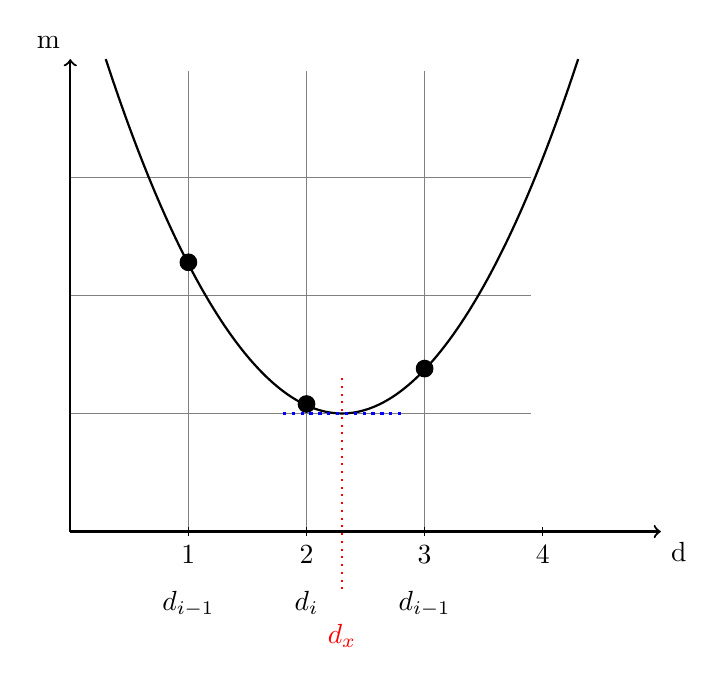
\begin{tikzpicture}[scale=1.5]
    %grid
    \draw[step=1cm,gray,very thin] (0,0) grid (3.9,3.9);
    %axes
    \draw[thick,->] (0,0) -- (5,0) node[anchor=north west] {d};
    \draw[thick,->] (0,0) -- (0,4) node[anchor=south east] {m};
    \foreach \x in {1,2,3,4}
      \draw (\x cm,1pt) -- (\x cm,-1pt) node[anchor=north] {$\x$};
    \draw (1cm,-12pt) node[anchor=north] {$d_{i-1}$};
    \draw (2cm,-12pt) node[anchor=north] {$d_{i}$};
    \draw (3cm,-12pt) node[anchor=north] {$d_{i-1}$};
    
    \draw[red] (2.3cm,-20pt) node[anchor=north] {$d_x$};
    %parabola
    \draw[thick] (2.3,1) parabola (0.3,4);
    \draw[thick] (2.3,1) parabola (4.3,4);
    %points
    \draw (1,2.28) circle[radius=2pt];
    \fill (1,2.28) circle[radius=2pt];
    \draw (2,1.08) circle[radius=2pt];
    \fill (2,1.08) circle[radius=2pt];
    \draw (3,1.38) circle[radius=2pt];
    \fill (3,1.38) circle[radius=2pt];
    %lines
    \draw[dotted,blue,very thick] (1.8,1) -- (2.8,1);
    \draw[dotted,red,thick] (2.3,1.3) -- (2.3,-0.5);
  \end{tikzpicture}
  \caption{Sub pixel estimation of a disparity value around adjacent pixels.}
  \label{fig:sub-pixel-estimation}
\end{figure}

\section{Optical flow}

Similar to the problems discussed in the section before, optical flow is also an image matching problem.
Optical flow is compiled of vectors describing small local displacements like moving objects or caused by the camera between two consecutive frames \citep{cyganek2011introduction, opencv_library}.
The principle of image matching like in disparity algorithms remains.
The main difference is that instead of analyzing left and right image, a scene is investigated and the disparity describes small local vectors.
To be more precise: it relies on the assumption that a certain point $(x_1, y_1)$ in a frame at time $t_1$ will be matched to a point $(x_2, y_2)$ in a frame at time $t_2$.
Different approaches for estimating the optical flow of pixels exist, like:

\begin{itemize}
  \item Correlation or block-matching,
  \item feature tracking,
  \item energy-based methods,
  \item gradient-based methods.
\end{itemize}

\begin{figure}[h!]
  \centering
  \includegraphics[width=0.9\textwidth]{src/images/optical-flow-estimation.jpg}
  \caption[Optical flow estimation]{Optical flow estimation to obtain motion vectors (left) and pixel velocity magnitudes (right).\protect\footnotemark}
  \label{fig:optical-flow-estimation}
\end{figure}
\footnotetext{Source (accessed 02/2016): \url{http://de.mathworks.com/discovery/optical-flow.html}.}

\noindent Optical flow is heavily used in autonomous driving, automated traffic surveillance systems and video compression, for instance: H.264 \citep{cohen1999detecting, richardson2004h, kondermann2015stereo, menze2015object}.
Recently a dataset containing ground-truth data of real-world sceneries regarding optical-flow information was released by \citeauthor{kondermann2015stereo}.
Figure \ref{fig:optical-flow-estimation} shows an example of estimating the movement of a vehicle.


\chapter{Related work}
\label{chap:related}

In this chapter the related work regarding disparity algorithms is treated.
As integration of some disparity algorithms for the later evaluation was part of this thesis, the ones which were actually implemented are examined in more detail.
The well-known semi-global matcher by \citeauthor{hirschmuller2005accurate} is introduced and the OpenCV implementations are mentioned.
An approach by \citeauthor{Geiger2010ACCV} to enable fast matching of high-resolution images is discussed.
Both approaches utilize local methods for estimating disparity maps.
One candidate adopting global methods is the Middlebury MRF library, which is also introduced in this chapter.
This implies solving optimization problems (i.e. the minimization of a global energy cost function).
Thus, the methods implemented by the library to solve such optimization problems are outlined.
In the end, a short outlook on spatiotemporal consistency regarding disparity algorithms applied on videos is presented.

\section{Semi-global matching}

\citeauthor{hirschmuller2005accurate} combines two different methods, global- and local-matching for determining accurate disparity at a lower runtime as other global algorithms, which tend to run pretty long on current hardware \citep{hirschmuller2005accurate, hirschmuller2008stereo}.
\newline\newline\noindent The semi-global matching (SGM) method utilizes pixel-wise matching of so called mutual information (MI) via entropy $H$, their joint-entropy of a pair of images and combining those with the approximation of a global two-dimensional smoothness constraint:

\begin{equation}
  MI_{I_1,I_2} = H_{I_1} + H_{I_2} + H_{I_1,I_2}.
\end{equation}

\noindent The previous discussed one-dimensional constraints are applied as well.
Calculating the matching cost based on mutual information is insensitive to recording differences and illumination changes \citep{hirschmuller2005accurate, viola1997alignment}.
The joint entropy $H_{I_1,I_2}$ is low (meaning low information content) for rectified images as one image can be predicted by the other.
The MI matching cost are defined as the following:

\begin{equation}
  mi_{I_1,I_2}(i,k) = h_{I_1}(i) + h_{I_2}(k) - h_{I_1,I_2}(i,k),
\end{equation}

\noindent where $h_1$ and $h_2$ are calculated from the probability distribution of corresponding intensities.
Thus, $h_{I_1,I_2}(i,k)$ serves as the matching cost for the two intensities $i$ and $k$.
The idea then is, that one image needs to be warped\footnote{In this context warping can be seen as a function which maps pixels from the destination image to pixels in the original image. Then the pixels are copied at the mapped position to the coordinates in the destination image.} such that corresponding pixels are at the same location in both stereo images:

\begin{equation}
    I_1 = I_b\quad \textrm{and}\quad I_2 = f_D(I_m),
\end{equation}

\noindent where $I_b$ is the base image, $I_m$ the match image and $f_D(x)$ is a function which outputs the matching corresponding point.
As the matching cost represent the information content of two intensities $I_1$ and $I_2$, which should be low (i.e. as equal as possible), the disparity map $D$ needs to be known \textit{a priori} for warping.
Hence, the MI matching cost needs to be calculated either iteratively or hierarchically.
On the one hand, an iteratively approach utilizes a random disparity image for calculating the MI matching cost, which serves as the base for the next iterations.
On the other hand, the MI matching cost can be calculated hierarchically by recursively using an up-scaled disparity image, which has been calculated at half resolution with a common similarity measurement like SAD.
For a deeper explanation of how the mutual information are exactly calculated and used in the SGM method compare \citep{hirschmuller2005accurate, hirschmuller2007evaluation, hirschmuller2008stereo, hirschmuller2011semi}.

\subsection*{OpenCV BM and SGBM}

The OpenCV library \citep{opencv_library} offers with its current version 3.1.0 two implementations for disparity estimation, block matching and semi-global block matching based on the idea of \citeauthor{hirschmuller2005accurate}.
This version also contains a new filter, which was initially introduced with version 3.0.0, named \textit{Disparity WLS Filter}\footnote{\url{http://docs.opencv.org/3.1.0/d9/d51/classcv_1_1ximgproc_1_1DisparityWLSFilter.html}}.
WLS stands for weighted least squares (in the form of a fast global smoother).
This disparity filter smoothes the disparity and also performs a left-right-consistency check to refine the results in especially half-occluded and uniform areas \citep{min2014fast}.
This yields to better and more accurate results but has the drawback of loosing negative disparity values.
Negative disparity can appear if the stereo cameras are verged or inclined towards each other.
The WLS filtering results in disparity ranging from $0$ to $D_{max}$, as set before.
Thus the negative disparity is $-1$.

\section{ELAS: Efficient large-scale stereo matching}

\citeauthor{Geiger2010ACCV} proposed a novel approach for estimating the disparity with so called support points \citep{Geiger2010ACCV, Geiger2011IV}.
A support point is like a feature, a point which can be robustly matched.
For those support points a sparse disparity map is calculated.
For more robustness, only the support points which can be matched left-to-right and right-to-left are retained.
To remove ambiguities, the ratio between the best and the second best match of all points is taken into account.
If the ratio exceeds a fixed threshold, the points are removed.
Support points which have a different disparity value than all adjacent points are outliers and removed as well.
As the found support points may not cover the whole image, additional support points in the image corners are added.
They adopt the disparity value of their nearest neighbor.
Then, image coordinates of the remaining support points are used to create a 2D mesh via Delaunay triangulation.
To obtain a dense disparity map missing disparities are interpolated using mesh of the Delaunay triangulation by using the nearest-neighbor on the same image line.
For more information how the support points get calculated and how the interpolation is done exactly, compare \citep{Geiger2010ACCV, Geiger2011IV}.

\section{Middlebury MRF library}

The Middlebury MRF library \citep{scharstein2014high, szeliski2008comparative} utilizes a global energy function consisting of Markov random fields to formulate an energy minimization problem and offers the following methods to solve this optimization problem:

\begin{enumerate}
  \item iterated conditional modes (ICM),
  \item graph cuts expansion approach (cf. \citep{boykov2001fast, ramin2004energy, kolmogorov2004energy}),
  \item graph cuts swap approach (cf. \citep{boykov2001fast, ramin2004energy, kolmogorov2004energy}),
  \item sequential tree-reweighted max-product message passing (TRWS)\\(cf. \citep{kolmogorov2006convergent, wainwright2005map}),
  \item sequential belief propagation (BPS) (cf. \citep{boykov2001fast}),
  \item max-product belief propagation (BPM) (cf. \citep{boykov2001fast}).
\end{enumerate}

\noindent The following subsections give a rough overview on some of those methods.
Additionally, a short introduction into MRF-based energy functions is given.
Also, the generalized concepts of how the above techniques help to solve such optimization problems are outlined.

\subsection{Solving optimization problems}

Many problems in computer vision can be described in terms of energy minimization for instance image smoothing, the stereo correspondence problems as described in Chapter \ref{chap:foundations} and many other.
Thus, solving of optimization problems is a key part in modern stereo matcher algorithms.
They solve the labelling problem as described in Chapter \ref{chap:foundations}.
Most of the current disparity algorithms are using global methods to solve an energy minimization problem.
Usually they utilize Markov random fields (MRF) based energy functions.
As such MRF based energy functions are \textit{NP-hard} approximation algorithms like the following are typically used \citep{tappen2003comparison, cyganek2011introduction}:

\begin{itemize}
  \item dynamic programming,
  \item belief propagation,
  \item graph cuts.
\end{itemize}

\noindent All of these methods have in common that they are supposed to solve so called inference problems, or at least approximate those.
Markov random fields, mentioned before, is also called Markov network.
Bayesian networks as well as Markov networks are so called graphical models.
Such graphical models help to understand the reasoning behind those formulations and to actually build algorithms which solve those inference problems.
Both networks express the dependencies of nodes as the conditional probability.
A chain of nodes is the so called joint probability.
This is then the product over-all (joint) probabilities.
The goal of algorithms which solve inference problem is to compute certain marginal probabilities, i.e. the probability that some pixel reaches a specific label node \citep{cyganek2011introduction}.
With inference the computation of these marginal probabilities is meant.
Marginal probabilities are defined as the sums over all possible state of all the other nodes in the system.
They are also called beliefs \citep{yedidia2003understanding}.

\subsubsection{Markov random fields}

Markov random fields (MRF), also called Markov network, are used to formulate problems in a probabilistic way represented as an undirected graph consisting of random variables, see \ref{fig:markov}.
A MRF is a graph $G = (V, E)$ with $V = {1,2,...N}$ denotes a set of vertices or nodes.
Each node is associated with a random variable $u_j$ for $j = 1...N$.
$E$ describes the edges $(i,j) \in E$ between the nodes $i$ and $j$.
The neighborhood of a node $i$ is the set of nodes to which the node $i$ is adjacent, i.e. $j \in N$ if and only if $(i,j) \in E$.
The neighborhood of a node $i$ is denoted as $N_i$.
For a simple undirected graph compare Figure \ref{fig:simple-graph}.

\begin{figure}[h!]
  \centering
  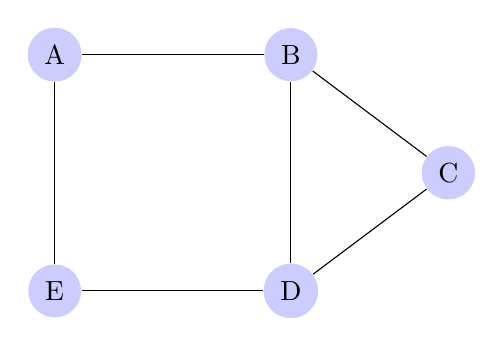
\begin{tikzpicture}
    [scale=1.0,auto=left,every node/.style={circle,fill=blue!20}]
    \node (nA) at (5,9)  {A};
    \node (nB) at (8,9)  {B};
    \node (nC) at (10,7.5) {C};
    \node (nD) at (8,6)  {D};
    \node (nE) at (5,6)  {E};
  
    \foreach \from/\to in {nA/nE,nA/nB,nB/nC,nC/nD,nD/nB,nD/nE}
      \draw (\from) -- (\to);
  \end{tikzpicture}
  \caption[Simple undirected unweighted graph]{Simple undirected unweighted graph}
  \label{fig:simple-graph}
\end{figure}

\noindent The Markov random field satisfies:

\begin{equation}
  P(u_i\ |\ \{u_j\}_{j \in V\\N}) = P(u_i\ |\ \{u_j\}_{j \in N_i}),
\end{equation}

\noindent where $N_i$ is the so called Markov blanket of node $i$.
It describes that the graph should be conditionally independent of all of the other variables given its neighbors.
A hop from one node to another can be seen as a chain of probabilities which have to occur, also called Markov chain.
The main idea behind MRF in combination with computer vision problems is to formulate the so called labelling problem in such a way, that each pixel has a likelihood to belong to a certain label \citep{tamassia2013handbook}.
The core problem then is to find exactly one label for each pixel, represented as a node in a MRF.
This label represents then the optimal solution to an underlying problem, in the case of stereo correspondence, the disparity for a pixel \citep{cyganek2011introduction}.
\newline\newline\noindent In contrast to MRF there also exist Bayesian networks.
A Bayesian network is a directed graph there as MRF is undirected.
This implies two important aspects, the direction of a certain probability to hop from one node to another.
MRF can not represent induced and non-transitive dependencies.
Two independent random variables may be connected by an edge because of possible dependencies.
Bayesian networks overcome this limitations.
\newline\newline\noindent The underlying stereo model of the Middlebury MRF library is based on the research of \citeauthor{sun2003stereo}.
They model stereo matching by three coupled MRF \citep{sun2003stereo}:
\begin{itemize}
  \item $D$ as the smooth disparity field,
  \item $L$ for representing depth-discontinuities,
  \item $O$ is a spatial binary state for handling occlusions.
\end{itemize}
\noindent Figure \ref{fig:mrf-stereo-matching} depicts the relationship between $D$, $L$ and $O$.
The joint probability over $D$, $L$ and $O$ given a pair of stereo images $I = {I_L,I_R}$ is defined as:
\begin{equation}
  P(D,L,O|I) = \frac{P(I|D,L,O)P(D,L,O)}{P(I)}.
\end{equation}
They then approximate inference via belief propagation over this equation.
For a deeper dive into this topic compare \citep{sun2003stereo, tamassia2013handbook, cyganek2011introduction, yedidia2003understanding, boykov2001fast, kolmogorov2006convergent, wainwright2005map}.

\begin{figure}[h!]
  \centering
  \includegraphics[width=1.0\textwidth]{src/images/mrf-stereo-matching.png}
  \caption[Stereo matching model by three coupled MRF's]{Stereo matching model by three coupled MRF's\citep{sun2003stereo}}
  \label{fig:mrf-stereo-matching}
\end{figure}

\subsubsection{Factor graph}

\noindent As those problems are \textit{NP-hard}, there exist several approximation algorithms which are outlined in the following subsections.
All of these approximation algorithms work on so called factor graphs.
A factor graph represents a factorized function and is bipartite\footnote{If the nodes of a graph can be divided into two disjoint sets, for instance $U$ and $V$, such that every edge connects a node $U$ to one in $V$, then the graph is bipartite.}.
A MRF function is factorized in partial functions and then formulated in a factor graph.
The solution to the problem represented by the factor graph is then approximated.
An important notion of factor graphs is the message which can be passed from a node to another.
There a few exceptions: for instance if the factor graph contains no cycles, the solution can then be exact computed with message passing algorithms (also called belief propagation) which work on a tree.
Otherwise only an approximation is possible.

\subsubsection{Dynamic programming}

In general, dynamic programming means having an optimization problem which can be parted into smaller chunks.
Then these chunks get solved individually and in the end, these chunks are connected and the optimization problem is minimized \citep{angel1972dynamic, bellman2015applied, cyganek2011introduction}.
For stereo matching this applies to the partition of a two-dimensional search problem into a series of isolated one-dimensional search problems on each pair of epipolar lines.
These problems are then solved independently.
With dynamic programming the following energy function (introduced in the foundations Chapter \ref{chap:foundations} can be solved independently per scanline.

\begin{equation}
  E(d) = E_{data}(d) + \lambda E_{smooth}(d)
\end{equation}

\noindent Dynamic programming has two benefits, it is solvable efficiently in polynomial time and it enforces the ordering constraint (as it is solved per scanline).
But it can lead to streaking effects, meaning that the result image seems to be constructed of many independent layers.

\subsubsection{Belief propagation}

Belief propagation (BP) is in general a technique to perform inference on a probabilistic model like Bayesian networks or Markov random fields \citep{yedidia2003understanding, tappen2003comparison, cyganek2011introduction}.
As mentioned before, \citeauthor{sun2003stereo} presented a stereo model for belief propagation.
BP works with messages which are passed from one node to another.
This is the reason why BP is also known as the message-passing algorithm.
The nodes exchange information about probabilities.
In the case of stereo matching, the message contains the probability that the receiver node (a node in MRF) should hold a disparity which is consistent with all information already passed to it by a sender.
The nodes are partitioned into low- and high-confidence ones.
The messages also carry a property, the entropy.
The entropy is high when sending from low- to high-confidence nodes and vice versa.

\subsubsection{Graph cuts}

For approximating problems formulated in a Markov random field there also exist so called graph cuts algorithms \citep{boykov2001fast, cyganek2011introduction}.
In general, graph cuts work like the following: assuming a graph $G$ with nodes $N$ and some edges $E$.
The goal is to delete enough edges so that each pixel is connected to exactly one label node.
Given a weighted graph $G$ with source $s$ and sink $t$ nodes.
The graph should be partitioned into two sets, $S$ and $T$, where $s \in S$ and $t \in T$.
This set presents a subgraph such that the sum of edge weights spanning this partition is minimized.
\newline\newline\noindent In the case of computer vision graph cuts are inspired by the combinatorial optimization methods for maximum flow \citep{cyganek2011introduction, cormen2009introduction}.
There exist two basic variations of the maximum flow problem, called $\alpha$-$\beta$-swap and $\alpha$-expansion.
Initially, three labels exist, that are $\alpha$, $\beta$ and $\lambda$. 
Normally, one step would be to change the label of a pixel, calculate the energy again and then infer if the change was good or not, depending on the delta.
For instance one pixel labelled with $\lambda$ would then be $\beta$.
The $\alpha$-$\beta$-swap algorithm whole areas of $\alpha$ are swapped with $\beta$ with $\lambda$ being unchanged.
In an $\alpha$-expansion a huge number of pixels labelled $\beta$ and $\lambda$ are changed into $\alpha$.
But in each of those methods the outcome is then measured.
In the foundations Chapter \ref{chap:foundations} the following equation was introduced:
\begin{equation}
  D = \arg\min_{d} E(d).
\end{equation}
\noindent If the outcome of such a swap or expansion is better, meaning $E(D_{after}) < E(D_{before})$, the algorithm continues.
If not, the algorithm stops.
Thus, both algorithms are expected to be stopped after the first unsuccessful run (i.e. energy increases).
The difficulty is to find the optimal swap move and the initial seed.
Both is described in \citep{boykov2001fast, sinha2004graph, tappen2003comparison, ramin2004energy}.

\section{Spatiotemporal consistency}

Although stereo correspondence is a research field which has been heavily investigated for a few decades no real disparity algorithm for videos exists yet.
One reason for that can be the lack of solid ground-truth data.
Only a few datasets has been introduced lately \citep{Butler:ECCV:2012, scharstein2014high}.
However, a novel approach was presented by \citep{richardt2010real}, \citep{khoshabeh2011spatio} and \citep{hosni2012temporally}.
\newline\newline\noindent The basic idea behind all of those presented approaches is to handle occurring noise.



Explain how the video restoration algorithms work (basically). They added noise. Blablabla.

\begin{itemize}
  \item Small description what is currently available.
  \item What can we do?
  \item Explain why some stuff is not available at all.
  \item Also point out the lack of ground truth data. This is a huge problem.
  \item Link to datasets!
\end{itemize}

Also outline the following approach: \citep{lee2012local}.



\chapter{Implementation}
\label{chap:impl}

Chapter \ref{chap:related} pointed out that no real algorithm for stereoscopic video disparity exist yet.
Other issues for more research in that area are:

\begin{itemize}
  \item No evaluation engine for videos exist yet.
  \item Currently only little datasets regarding ground-truth data for stereoscopic videos are available.
\end{itemize}

\noindent Thus, the decision towards an own evaluation engine was made.
In this chapter the implementation, its components and the novel approach concerning the subsequent optimization of disparity maps are described.

\section{Preliminaries}

As development platform a MacBookPro was used with the following specifications: i5-4258U CPU @ 2.40GHz, 8 GB RAM, a fast SSD.
Everything except the web result viewer was implemented using C++.
As a timer saver and for reducing code duplicates OpenCV as master library was used.
Everything is based on OpenCV.
In addition the Boost library was used for some simple tasks like creating an array of arbitrary length for keeping a simple binary state or parsing the command line options.
The build-chain consists of some shell scripts and CMake as makefile generator.
With CMake it was possible to cross-compile the app for Linux and use a fast server-instance from DigitalOcean\footnote{\url{https://www.digitalocean.com}} for the generation of the disparity maps and to actually evaluate those.
\noindent Especially a docker image was created\footnote{\url{https://github.com/benjohnde/dockerbase-opencv}}.

%todo describe docker image and deployment
%todo describe desktop tower
%todo python scripts for evaluation were used
%todo some fun facts like the overall evaluation time needed
%todo the amount of processed data

\section{Overview}

\tikzstyle{rblock} = [text width=9em, rectangle, draw, fill=blue!18, text centered, rounded corners, minimum height=4em]
\tikzstyle{cloud} = [text width=6em, ellipse, draw, fill=blue!6, text centered, rounded corners, minimum height=3.2em]
\begin{figure}[h!]
  \centering
  \begin{tikzpicture}[node distance=7em, auto]
    %input
    \node [cloud] (right) {right image};
    \node [cloud, right of=right, node distance=10em] (left) {left image};
    \node [cloud, right of=left, node distance=10em] (disp) {ground-truth};

    %computation
    \node [rblock, below of=right, xshift=2em] (exec) {(1) Algorithm executer};
    \node [rblock, below of=disp, xshift=-2em] (mask-creator) {(2) Mask creator};

    %output
    \node [cloud, below of=exec] (map) {disparity map};
    \node [cloud, below of=mask-creator] (masks) {masks};

    %evaluation
    \node [rblock, below of=left, yshift=-14em] (evaluation) {(3) Disparity evaluator};

    %final result
    \node [cloud, below of=evaluation, xshift=-5em] (csv) {csv file};
    \node [cloud, below of=evaluation, xshift=5em] (heatmaps) {heatmaps};

    %lines
    \path [line] (right) -- (exec);
    \path [line] (left) -- (exec);
    \path [line] (left) -- (mask-creator);
    \path [line] (disp) -- (mask-creator);

    \path [line] (exec) -- (map);
    \path [line] (mask-creator) -- (masks);

    \path [line] (map) -- (evaluation);
    \path [line] (masks) -- (evaluation);

    \path [line] (evaluation) -- (csv);
    \path [line] (evaluation) -- (heatmaps);
  \end{tikzpicture}
  \caption{Processing pipeline of the implementation.}
  \label{fig:impl-pipeline}
\end{figure}

%todo describe evolution
%todo describe general flow
%todo describe why it was built
%todo describe folder structure
%todo describe OpenEXR file format
%todo describe csv format of output
%todo create uml diagrams for basic implementation

\noindent Initially, a rapid monolithic prototype was built featuring the execution of different disparity algorithms, the creation of bitmasks and the evaluation of a given scene with different parameters.
But as more datasets were found and various bitmasks as an evaluation method were established the need for a leaner process chain arose.
Especially as disparity algorithms need some time to compute the disparity map for one frame.
Hence, as videos consist of multiple frames (in our datasets about 90 frames in mean) this is a time consuming task.
Sometimes metrics change or a new metric is established, the threshold can be adjusted.
These are the reasons for an approach towards microservices with which computed disparity maps can be evaluated repeatedly and independently.
Thus, the monolith was rewritten partitioned in smaller microservices shaping three different components:

\begin{itemize}
  \item disparity algorithm executer,
  \item mask creator,
  \item evaluation engine.
\end{itemize}

\noindent The figure \ref{fig:overview-uml} shows the composition and figure XXX the evaluation chain of these microservices.
The output which each one of those microservices in the chain can generate or operate on is structured in a simple folder tree:

\begin{itemize}
  \item /datasets/\{dataset\_identifier\}/\{dataset\_sequence\_identifier\}/\{appendix\}
\end{itemize}

\noindent There \{appendix\} can be either \{disparity\_maps\_computed\}, \{disparity\_maps\_smoothed\} or \{bitmasks\}.
\newline\newline\noindent The computed disparity maps are saved in a binary format since OpenCV is currently not able to use the OpenEXR file format properly (only reading is possible).
Hence for visualization they have to be normalized in the range of 0-255 or may be presented as a heat map.
The evaluation is done with simple python scripts reflecting the evaluation chain.

\begin{figure}[h!]
  \centering
  \begin{tikzpicture}

    %classes
    \umlclass[x=0,y=0]{OpenCVStereoBM}{}{}
    \umlclass[x=0,y=3,type=interface]{DisparityAlgorithm}{}{}

    \umlclass[x=5,y=0]{NaiveSmoothing}{}{}
    \umlclass[x=5,y=3,type=interface]{SmoothingAlgorithm}{}{}

    \umlclass[x=2.5,y=6]{EvalSuite}{}{- evaluateFrame()\\- evaluateFrames()}

    \umlclass[x=2.5,y=9]{Metrics}{}{}

    %connections
    \umlassoc{EvalSuite}{Metrics}

    \umluniassoc{DisparityAlgorithm}{EvalSuite}
    \umluniassoc{SmoothingAlgorithm}{EvalSuite}

    \umlimpl{OpenCVStereoBM}{DisparityAlgorithm}
    \umlimpl{NaiveSmoothing}{SmoothingAlgorithm}

  \end{tikzpicture}
  \caption{Simplified UML diagram of general architecture.}
  \label{fig:overview-uml}
\end{figure}

\begin{figure}[h!]
  \centering
  \begin{tikzpicture}

    %classes
    \umlclass[x=2,y=0]{EvalResultMetric}{}{}
    \umlclass[x=0,y=3]{FrameResult}{}{}
    \umlclass[x=4,y=3]{EvalResult}{}{}

    %connections
    \umluniassoc{EvalResultMetric}{FrameResult}
    \umluniassoc{FrameResult}{EvalResult}

    \umluniassoc{EvalResultMetric}{EvalResult}
  \end{tikzpicture}
  \caption{Simplified UML diagram of result composition for further processing.}
\end{figure}

%todo another uml diagram with the following:
%\umlclass{EvalResult}{}{}
%\umlclass{FrameResult}{}{}
%\umlclass{EvalResultMetric}{}{}

\section{Evaluation engine for videos}

At the current point in time, no real disparity algorithm for especially videos exists yet.
As a video is defined by multiple consecutive frames, every disparity algorithm for images can be applied on videos.
The drawback of this trivial approach is the lack of taking the correlation of the frames into account.
None the less it is possible to focus on some other details, for instance:

\begin{itemize}
  \item possible outliers in the sense of frames,
  \item mean performance (error rate) of those algorithms on a complete scene,
  \item runtime variety in a sequence,
  \item analyzing the impact of noise, and
  \item trying to smooth noisy areas in the resulting disparity map with other frames.
\end{itemize}

\noindent Noise can occur through video compression.
As video sensors tend to be noisier than image sensors it also more present in stereoscopic videos, if not rendered by a computer.
As noise can be simulated and added onto the rendered video, it is investigated how noise disturb stereo matcher.
As these ideas are more explained in the implementation chapter \ref{chap:impl} the following subsection a novel approach for videos are examined.

In contrast to other implementations, input and output are clearly defined and thus different techniques can be adapted easily.
There exist combined frameworks which fulfill two tasks, disparity calculation (as the algorithm is implemented) and the final evaluation step.
This makes it harder to use the evaluation module separately from the rest.
None the less the open source community around computer vision also lacks of code for stereo matcher.
Due the diversities of algorithms and eval suites the decision was made to go for an OpenCV implementation of an eval suite for disparity algorithms.

%todo
Works basically as a wrapper. Can output statistical stuff. Basically works on disparity maps / images.

Huge mistake could be to apply the metrics on the whole disparity map from the algorithm. The output contains areas which are black (value = 0). This can be:

\begin{itemize}
  \item noise
  \item mistaken be the algorithm
  \item expected disparity
  \item non-occluded areas
\end{itemize}

\tikzstyle{block} = [rectangle, draw, fill=blue!20,
    text width=5em, text centered, rounded corners, minimum height=4em]
\tikzstyle{line} = [draw, -latex']
\tikzstyle{cloud} = [draw, ellipse,fill=red!20, node distance=4cm,
    minimum height=2em]

\begin{center}
\begin{tikzpicture}[node distance = 2cm, auto]
    \node [block] (init) {initialize eval engine with input};
    \node [cloud, left of=init] (gt) {ground-truth data};
    \node [cloud, right of=init] (ao) {algorithm output};
    \node [block, below of=init] (calc) {calculate differences};
    \node [block, below of=calc] (evaluate) {apply statistical methods};
    \node [block, below of=evaluate] (output) {output};

    \path [line] (init) -- (calc);
    \path [line] (calc) -- (evaluate);
    \path [line] (evaluate) -- (output);
    \path [line, dashed] (gt) -- (init);
    \path [line, dashed] (ao) -- (init);
\end{tikzpicture}
\end{center}

The eval engine has two modes to be queried:

\begin{itemize}
  \item via command-line which also results in a console output,
  \item with a configuration file ($config.json$) which leads to an output in a given folder for the web result viewer.
\end{itemize}

\subsection*{Preprocessing}

Different tasks are executed before the actual disparity algorithm are invoked and the evaluation takes place:

\begin{itemize}
  \item Normalization
  \item Gaussian noise
\end{itemize}

\subsection*{Postprocessing}

Postprocessing only consists of one task: normalization of the disparity map.
Some algorithms struggle with calculating a larger number than the number of disparities of $32$.
Some datasets only calculated the disparity to be in a range from $0$ to $63$.
Grayscale normally ranges from $0$ to $255$.
Thus the disparity map is normalized to range from $0$ to $63$.

Simply only disparity normalization.

\section{Fine-grained evaluation via masks}

The evaluation would be trivial by just comparing the computed disparity map with its ground-truth companion.
This trivial comparison would be a pitfall, as the results would be erroneous due to for instance unknown disparity or occluded regions.
As remedy bitmasks are introduced to simply focus on interesting pixels.
In this section the following bitmasks are introduced and how they are calculated:

\begin{itemize}
  \item Depth-discontinuity
  \item Textured regions recognition
  \item Discover occluded pixels
  \item Saliency detection
  \item Unknown disparity
\end{itemize}

%todo motivational introduction to bitmasks
First describe the motivational introduction to bitmasks why would one use those?

\subsection*{Depth-discontinuity}

Determining correspondence can fail in textureless or depth-discontinuous regions as mentioned above.
Thus it is also interesting how the algorithms handle such regions. For this purpose a depth-discontinuity mask was implemented as well.

Explain:

\begin{itemize}
  \item Dilate
  \item Erode
  \item maybe show short example image (combined dilate/erode)
  \item explain how the bitmask is calculated
\end{itemize}

\subsection*{Textured regions recognition}

As stereo matching algorithms act on the assumption that the disparity is smooth, especially if contrast and color intensity do not change drastically, it can be interesting to see how those algorithms treat textured and textureless regions.
Thus a bitmask for textured regions recognition was implemented.

Explain (shortly):

\begin{itemize}
  \item Sobel
  \item pow
  \item boxFilter
  \item how we get the bitmask
\end{itemize}

\subsection*{Discover occluded pixels}

An occluded pixel is defined as a pixel which is hidden in one of the two images, for instance an object hides it from a different angle.
In the case of stereo matching the disparity can not be calculated for such a pixel.
Thus occluded pixels have to be handled properly, as they could distort our result.
For this purpose a simple mask is introduced to indicate which pixels on the scene are visible for both cameras and which are not.

Explain and cite two papers (taxonomy of disparity algorithms).
There it is explained how everything is working.
Explain how the get the result (use algorithm).

Thus we need to take care about non-occluded areas. For this purpose we generated bitmasks (the size $w$ * $h$) for each video dataset.

"In addition to disparity maps, for stereo matching method evaluation it is interesting to have a non-occluded area mask. This mask represents in white color the pixels on the scene that are visible from both cameras and in black color the pixels that are visible from only one camera.
To obtain the non-occluded area mask, we simply cross-checked the left and right disparity maps. Pixels that are visible in both cameras will have the same value in both disparity maps, but for occluded pixels the left and right disparity value will be different.
The performance of the stereo matching algorithm on areas where pixels are occluded is one of the most important quality indicators of the algorithm, as it is very difficult to find the matching point of a pixel in one of the images if it is not visible on the other image." \citep{martull2012realistic}.

\subsection*{Saliency detection}

Another criteria for the later evaluation is how the algorithms operate on regions which are salient in a specific scene.
There exist some algorithms for saliency detection in either images or videos \citep{dittrich2013saliency, opencv_library}.
OpenCV offers two different saliency categories to be computed:
\begin{itemize}
  \item $StaticSaliency$ in images, and
  \item $MotionSaliency$ on videos.
\end{itemize}

\noindent Explain how saliency detection works, implemented via OpenCV. Otsu's algorithms, threshold and K-Means algorithm \citep{hou2007saliency}.

\section{Integration of existing algorithms}

Deciding which algorithms should be describe was not an easy task.
On the one hand, the algorithms which shall be implemented during this thesis are important and thus should be described definitely.
On the other hand, there is a huge diversity of used technologies amongst disparity algorithms.
For instance various programming languages, the decision between cpu- versus gpu-rendering, different coding styles and used libraries.
As a matter of fact, this makes it harder to implement and then evaluate every single disparity algorithm.
Thus, the algorithms from Middlebury were integrated in the evaluation suite and streamlined.
Additionally, the so called efficient large-scale stereo matcher (ELAS) was also integrated.
The parameters used for each algorithm are described in the implementation chapter.
This section is for giving an overview on these algorithms as well as their parameters for the later implementation chapter \ref{chap:impl}.

\tikzstyle{block} = [rectangle, draw, fill=blue!20,
    text width=5em, text centered, rounded corners, minimum height=4em]

\begin{figure}[h]
  \centering
  \begin{tikzpicture}[node distance = 3cm, auto]
    \node [block] (pre) {pre-processing};
    \node [block, right of=pre] (call) {call wrapper};
    \node [block, right of=call] (post) {post-processing};

    \path [line] (pre) -- (call);
    \path [line] (call) -- (post);
  \end{tikzpicture}
  \caption{Basic integration of existing algorithms}
  \label{fig:integration}
\end{figure}

This does not exist currently, so we use the Middlebury Test Suite with its algorithms for images and apply them on videos.

\begin{itemize}
	\item Consists of multiple steps
	\item Wrapper to call different algorithms
	\item normalizing of output
	\item actual eval process
\end{itemize}

Input: ImageLEFT, ExpectedLEFT, ImageRIGHT, ExpectedRIGHT
Output: a good metric for showing good/bad disparity, a few ideas.

\section{Image diminisher to simulate real use cases}

\subsection*{Gaussian noise}

randn\footnote{\url{http://docs.opencv.org/master/d2/de8/group__core__array.html\#gaeff1f61e972d133a04ce3a5f81cf6808}}

%todo finish chapter of gaussian noise

\citep{opencv_library}

As seen in the related work chapter \ref{chap:related}, some approaches use restoration algorithms in order to reduce noise which can occur.
Hence noise generation was added as a preprocessing step in order to see how noise disrupts disparity algorithms.
We use gaussian noise meaning that the noise is gaussian-distributed.

$$f\left(x\right) = a e^{- { \frac{(x-b)^2 }{ 2 c^2} } }$$

$$p_G(z) = \frac{1}{\sigma\sqrt{2\pi}} e^{ -\frac{(z-\mu)^2}{2\sigma^2} }$$

\noindent In this example, $z$ represents the grey level which is added to the image matrix later on.
$\mu$ is the mean value (= 0).
$\sigma$ is the standard deviation.
\newline\newline\noindent The $\sigma$ can be set in our evaluation suite in order to see how this distracts the image.

\pgfmathdeclarefunction{gauss}{2}{%
  \pgfmathparse{1/(#2*sqrt(2*pi))*exp(-((x-#1)^2)/(2*#2^2))}%
}

\begin{figure}[h!]
\center
\begin{tikzpicture}
\begin{axis}[every axis plot post/.append style={
  mark=none,domain=-2:3,samples=50,smooth}, % All plots: from -2:2, 50 samples, smooth, no marks
  axis x line*=bottom, % no box around the plot, only x and y axis
  axis y line*=left, % the * suppresses the arrow tips
  enlargelimits=upper] % extend the axes a bit to the right and top
  \addplot {gauss(0,0.5)};
  \addplot {gauss(1,0.75)};
\end{axis}
\end{tikzpicture}
\end{figure}

\subsection*{Video compression}

FFMPEG \citep{FFMPEG2010}.

\section{Web result viewer for evaluation suite}

For fine-tuning the algorithm's parameters as well as implementing the bitmasks it was helpful to see the visual output of both.
As the resulting bitmasks for each frame with the computed result disparity map were saved on the hard-drive for further investigations a web result viewer was created for visualizing the output.
The following features were implemented:
\begin{itemize}
  \item Starting new computations with different parameters and scene selection.
  \item Playing frame-by-frame with different speeds.
  \item Online csv-export of result.
\end{itemize}

\begin{figure}[p!]
  \centering
  \includegraphics[angle=90,width=0.7\textwidth]{src/images/result-viewer-overview.png}
  \caption{Overview page of web result viewer.}
  \label{fig:web-overview}
\end{figure}

\begin{figure}[p!]
  \centering
  \includegraphics[angle=90,width=1.0\textwidth]{src/images/result-viewer-detail.png}
  \caption{Detail of one result in the web result viewer.}
  \label{fig:web-detail}
\end{figure}

%todo finish web result viewer section
\begin{itemize}
  \item Insert screenshot (one or two from web result viewer)
  \item Describe basic features
  \item Describe what could be done with the evaluation web suite in near future
  \item But for thesis evaluation a csv exporter was used.
\end{itemize}

\section{Discussion}

The following modules were actually implemented:

\begin{itemize}
  \item Reader for the PFM file format.
  \item Python scripts for upcoming evaluation.
  \item Shell scripts for getting the docker containers and thus the work distributed among different instances\footnote{With instances virtual machines from DigitalOcean are meant.}.
  \item Evaluation processor for
\end{itemize}


\chapter{Evaluation and results}
\label{chap:eval}

%todo smooth me

In the previous chapter, the evaluation suite and its features were presented.
This chapter is split into several subtopics.
First, it deals with the introduction of datasets.
Second, the quality metrics for the comparison of disparity algorithms  for stereoscopic videos are defined.
Third, the structure of the measurement is illustrated.
Fourth, the results are visualized and discussed.
\newline\newline\noindent Overall, the setup for the evaluation took 24 days to process 30 GB of stereoscopic videos and to create all disparity maps.
Accumulated, the computed disparity maps, the created masks as well as the heatmaps, took about 8 GB.

\section{Datasets}

A dataset basically describes a set of stereo images, which additionally contains ground-truth disparity maps.
The aim of such datasets is to provide data which researchers can rely on, to evaluate the performance of computer vision algorithms, such as disparity algorithms in this thesis.
 Without having such datasets it would be crucial to rate the overall quality of for instance stereo matching algorithms.
As for today, no high-resolution stereoscopic video dataset exists yet, neither a synthetic nor a captured one.
In order to obtain ground-truth depth information, there exist in general two options.
On the one hand, the real-world can be sensed via area scanner, for instance a radar.
On the other hand, a synthetic computer-animated scene is generated and the renderer calculates the disparity.
Of course, the former approach is more error-prone than the latter one.
The former one can lack of accuracy due to false measurements whereas the latter one real ground-truth information provides.
\newline\newline\noindent \citeauthor{kondermann2015stereo} came up with an interesting approach.
As area scanners are never 100 percent accurate, they introduced error-bars, which can range from $0-10$.
An error-bar indicates how certain the area scanner was that this disparity for a given pixel really existed \citep{kondermann2015stereo}.
\newline\newline\noindent As it would be a tremendous task to evaluate every existing stereoscopic dataset with every existing disparity algorithms, here three different datasets were chosen.
As reference dataset, the reworked Tsukuba Stereo Dataset was chosen \citep{martull2012realistic}.
The scene is called \textit{Head and Lamp} and was also shortly introduced in the foundations Chapter \ref{chap:foundations}.
\newline\newline\noindent The second one is a dataset, especially created for the evaluation of the DCBGrid from the University of Cambridge\footnote{\url{http://www.cl.cam.ac.uk/research/rainbow/projects/dcbgrid/datasets/}}.
This is also one of the first stereoscopic dataset targeting videos.
As second dataset, a novel, not yet analyzed dataset was chosen: the SVDDD\footnote{SVDDD stands for a high-resolution Stereoscopic Video Dataset with precise Depth and Disparity information.} dataset.
The Lehrstuhl f{\"u}r Praktische Informatik IV\footnote{\url{http://ls.fmi.uni-mannheim.de/de/pi4/}} created the dataset on its own with high-resolution video sequences containing accurate depth and disparity information for stereoscopic videos.
%todo a bit more
Other datasets, which were found but not investigated further more are: MPI Sintel Stereo Training Data, created for optical flow evaluation \citep{Butler:ECCV:2012} and the Middlebury stereo dataset, providing real images with ground-truth information \citep{scharstein2006middlebury}.




\subsection{Tsukuba stereo dataset}

This dataset can be seen as the origin of stereoscopic datasets.
The first dataset ever released for working with stereoscopic images.
\citep{martull2012realistic}.

%todo intro

\subsection{Cambridge stereo dataset}

%todo intro

\begin{figure}[h!]
  \centering
  \includegraphics[width=1.0\textwidth]{src/images/dbcgrid-dataset.png}
  \caption[Middlebury stereo dataset example]{Middlebury stereo dataset example}
  \label{fig:dbcgrid-dataset}
\end{figure}

The Cambridge stereo dataset consists of five different rendered scenes in $400x300$ resolution with each about 100 frames \citep{richardt2010real}.
The dataset scales the disparity for each scene from $0$ to $64$.

\subsection{SVDDD - a high-resolution Stereoscopic Video Dataset with precise Depth and Disparity information}

The Lehrstuhl f{\"u}r Praktische Informatik IV\footnote{\url{http://ls.fmi.uni-mannheim.de/de/pi4/}} has created a novel dataset on its own containing depth information for stereoscopic videos.
Before the evaluation it was clear that this dataset is going to be evaluated as well.
The difference is that this dataset was not analyzed before.
Thus it is possible that the chosen algorithms work not properly on this dataset.
If this case occurs there exist two possibilities why this happens:

\begin{itemize}
  \item On the one hand, the disparity information are not properly calculated, or
  \item on the other hand, those algorithms have some troubles with the constructed scene.
\end{itemize}

\noindent Focusing on the latter one, the scenes were created with Blender and utilizes the XXX (insert me pls) open-source scenes.
A second camera was added to the scene for obtaining depth information.
The parameter for each scene can be extracted from the paper.
The most important points which can lead to a discrepancy between the computed disparity maps and the ground-truth data are the following:

\begin{itemize}
  \item rays of light were removed only in the ground-truth-data,
  \item motion and object blur was reduced only in the ground-truth data,
  \item fain-grained textures were reduced only in the ground-truth data.
\end{itemize}

%todo describe potential drawbacks
%todo go into more concrete

\section{Quality metrics}

To evaluate the quality of computed disparity maps we need at first to what we compare the computed disparity maps to and secondly how to compare them. In the section \ref{chap:datasets} the availability of such datasets were discussed.

Insert table here.

\begin{table}[h!]
\centering
\begin{tabular}{l|l}
\textbf{Tag} & \textbf{Description} \\ \hline
$\sigma_{10}$ & Guassian noise calculator. \\ \hline
 &  \\ \hline
 &  \\
\end{tabular}
\caption{Overview on used metrics in results}
\label{tab:metrics}
\end{table}

\noindent Typical quality measure instruments for comparing disparity maps against their ground-truth reference data are  \citep{cyganek2011introduction}:

\begin{itemize}
  \item Percentage of bad matching pixels
  \item Root-mean-square error
  \item Parameter-free measures
\end{itemize}

In addition the following are also considered:

\begin{itemize}
  \item Mean absolute error in pixels
  \item Error quantiles
  \item Precision and accuracy
\end{itemize}

\subsection*{Percentage of bad matching pixels}

\begin{equation}
  \operatorname{PBMP}=\frac{1}{n} \sum_{x,y=0}^{}(|d_a(x,y) - d_e(x,y)| > \delta_t)
\end{equation}

\noindent Percentage of bad matching pixels for given threshold.

\subsection*{Root-mean-squared error}

The mean squared error (MSE) as well as the root mean squared error (RMSE) are both the most popular metrics in image and video processing.
The MSE is as the name implies the mean of the squared differences between the intensities of pixels in two pictures at the same position.
In conclusion the average difference per pixel is then the root of the squared error.

\begin{equation}
  \operatorname{RMS-Error}=\sqrt{\frac{1}{n} \sum_{x,y=0}^{}(d_a(x,y) - d_e(x,y))^2}
\end{equation}

\noindent It represents the sample standard deviation of the differences between predicted values and observed values.
Here $d_a(x,y)$ is the actual disparity value for given $x$ and $y$.
$d_e(x,y)$ is our expected disparity value from our ground-truth data.
Hence the RMSE is the difference between values on average.

\section{Measurement}

\begin{itemize}
	\item First took normal depth map images. But not that good, only values from 0-255.
	\item Actual evaluation process consists of comparison of real calculated values of depth map by results of algorithms.
	\item How does the eval actual look like?
\end{itemize} \citep{benoit2008quality}, \citep{scharstein2002taxonomy}.

\subsection*{Parameter tuning}

Our results.

\subsection*{Against reference dataset}

It is also important to have some kind of reference dataset with which the evaluation engine can be calibrated with.
Of course the settings (i.e. parameters of an algorithm) is dependent on the input material (size, noise) and on the scene (e.g. textured vs textureless).
So it is possible to have good parameters for one scene and not for another.
However, in order to evaluate those algorithms the Tsubuka stereo dataset was chosen as reference dataset to see how the eval engine actually works with the same parameters on the same images.

\section{Results}

%todo small intro

The results are visualized with the HSV color model.

\begin{figure}[h!]
  \centering
  \includegraphics[width=0.8\textwidth]{src/images/hue-scale.png}
  \caption{Scale of hue of the HSV color model.}
  \label{fig:hue-scale}
\end{figure}

%todo results

\subsection*{Applying disparity algorithms on videos}

As said in the implementation chapter \ref{chap:impl} applying disparity algorithms on videos is trivial and straightforward.
None the less different anomalies can be further investigated while analyzing videos:

\begin{itemize}
  \item outliers in the form of a single frames which differs too much from the others,
  \item impact of noise,
  \item smooth the unknown disparity in frames (next subsection).
\end{itemize}

\noindent As you can see in the following result matrices the quality metrics regarding the salient regions are a bit esoteric. Of course there exist techniques to estimate salient regions in static images and also in videos. In videos moving objects can be detected as salient, referring to motion saliency\citep{opencv_library, wang2014fast}. None the less those bitmasks are a bit more esoteric in the sense of there is room for interpretation.

\begin{landscape}
  \begin{table}[h!]
  \centering
  \begin{tabular}{cll|rrrrr}
    \hline
    \textbf{Rank} & \textbf{Method} & \textbf{Sequence} & \textbf{RMS-All} & \textbf{RMS-Noc} & \textbf{RMS-Sal} & \textbf{RMS-Tex} & \textbf{RMS-DD} \\ \hline \hline
    1 & StereoSGBM & SVDDD 02\_rabbit & 4.35\% & \cellcolor{green!60}5.43\% & 1.0 px & 1.1 px & 300ms \\
    2 & StereoBM & SVDDD 02\_rabbit & 4.35\% & 5.43\% & 1.0 px & \cellcolor{red!60}1.1 px & 300ms \\ \hline
  \end{tabular}
  \caption{Result matrix of RMS for videos}
  \label{tab:result-videos-rms}
  \end{table}
\end{landscape}

\begin{landscape}
  \begin{table}[h!]
  \centering
  \begin{tabular}{cll|rrrrr}
    \hline
    \textbf{Rank} & \textbf{Method} & \textbf{Sequence} & \textbf{Out-All} & \textbf{Out-Noc} & \textbf{Out-Sal} & \textbf{Out-Tex} & \textbf{Out-DD} \\ \hline \hline
    1 & StereoSGBM & SVDDD 02\_rabbit & 4.35\% & \cellcolor{green!60}5.43\% & 1.0 px & 1.1 px & 300ms \\
    1 & StereoSGBM & SVDDD 02\_rabbit & 4.35\% & \cellcolor{green!60}5.43\% & 1.0 px & 1.1 px & 300ms \\
    1 & StereoSGBM & SVDDD 02\_rabbit & 4.35\% & \cellcolor{green!60}5.43\% & 1.0 px & 1.1 px & 300ms \\
    1 & StereoSGBM & SVDDD 02\_rabbit & 4.35\% & \cellcolor{green!60}5.43\% & 1.0 px & 1.1 px & 300ms \\
    1 & StereoSGBM & SVDDD 02\_rabbit & 4.35\% & \cellcolor{green!60}5.43\% & 1.0 px & 1.1 px & 300ms \\
    1 & StereoSGBM & SVDDD 02\_rabbit & 4.35\% & \cellcolor{green!60}5.43\% & 1.0 px & 1.1 px & 300ms \\
    1 & StereoSGBM & SVDDD 02\_rabbit & 4.35\% & \cellcolor{green!60}5.43\% & 1.0 px & 1.1 px & 300ms \\
    1 & StereoSGBM & SVDDD 02\_rabbit & 4.35\% & \cellcolor{green!60}5.43\% & 1.0 px & 1.1 px & 300ms \\
    1 & StereoSGBM & SVDDD 02\_rabbit & 4.35\% & \cellcolor{green!60}5.43\% & 1.0 px & 1.1 px & 300ms \\
    1 & StereoSGBM & SVDDD 02\_rabbit & 4.35\% & \cellcolor{green!60}5.43\% & 1.0 px & 1.1 px & 300ms \\
    1 & StereoSGBM & SVDDD 02\_rabbit & 4.35\% & \cellcolor{green!60}5.43\% & 1.0 px & 1.1 px & 300ms \\
    1 & StereoSGBM & SVDDD 02\_rabbit & 4.35\% & \cellcolor{green!60}5.43\% & 1.0 px & 1.1 px & 300ms \\
    1 & StereoSGBM & SVDDD 02\_rabbit & 4.35\% & \cellcolor{green!60}5.43\% & 1.0 px & 1.1 px & 300ms \\
    1 & StereoSGBM & SVDDD 02\_rabbit & 4.35\% & \cellcolor{green!60}5.43\% & 1.0 px & 1.1 px & 300ms \\
    1 & StereoSGBM & SVDDD 02\_rabbit & 4.35\% & \cellcolor{green!60}5.43\% & 1.0 px & 1.1 px & 300ms \\
    1 & StereoSGBM & SVDDD 02\_rabbit & 4.35\% & \cellcolor{green!60}5.43\% & 1.0 px & 1.1 px & 300ms \\
    1 & StereoSGBM & SVDDD 02\_rabbit & 4.35\% & \cellcolor{green!60}5.43\% & 1.0 px & 1.1 px & 300ms \\
    1 & StereoSGBM & SVDDD 02\_rabbit & 4.35\% & \cellcolor{green!60}5.43\% & 1.0 px & 1.1 px & 300ms \\
    1 & StereoSGBM & SVDDD 02\_rabbit & 4.35\% & \cellcolor{green!60}5.43\% & 1.0 px & 1.1 px & 300ms \\
    1 & StereoSGBM & SVDDD 02\_rabbit & 4.35\% & \cellcolor{green!60}5.43\% & 1.0 px & 1.1 px & 300ms \\
    1 & StereoSGBM & SVDDD 02\_rabbit & 4.35\% & \cellcolor{green!60}5.43\% & 1.0 px & 1.1 px & 300ms \\
    2 & StereoBM & SVDDD 02\_rabbit & 4.35\% & 5.43\% & 1.0 px & \cellcolor{red!60}1.1 px & 300ms \\ \hline
  \end{tabular}
  \caption{Result matrix of outliers for videos}
  \label{tab:result-videos-out}
  \end{table}
\end{landscape}



\begin{figure}[h!]
\centering
\begin{tabular}{cc}

\subfloat[Left image]{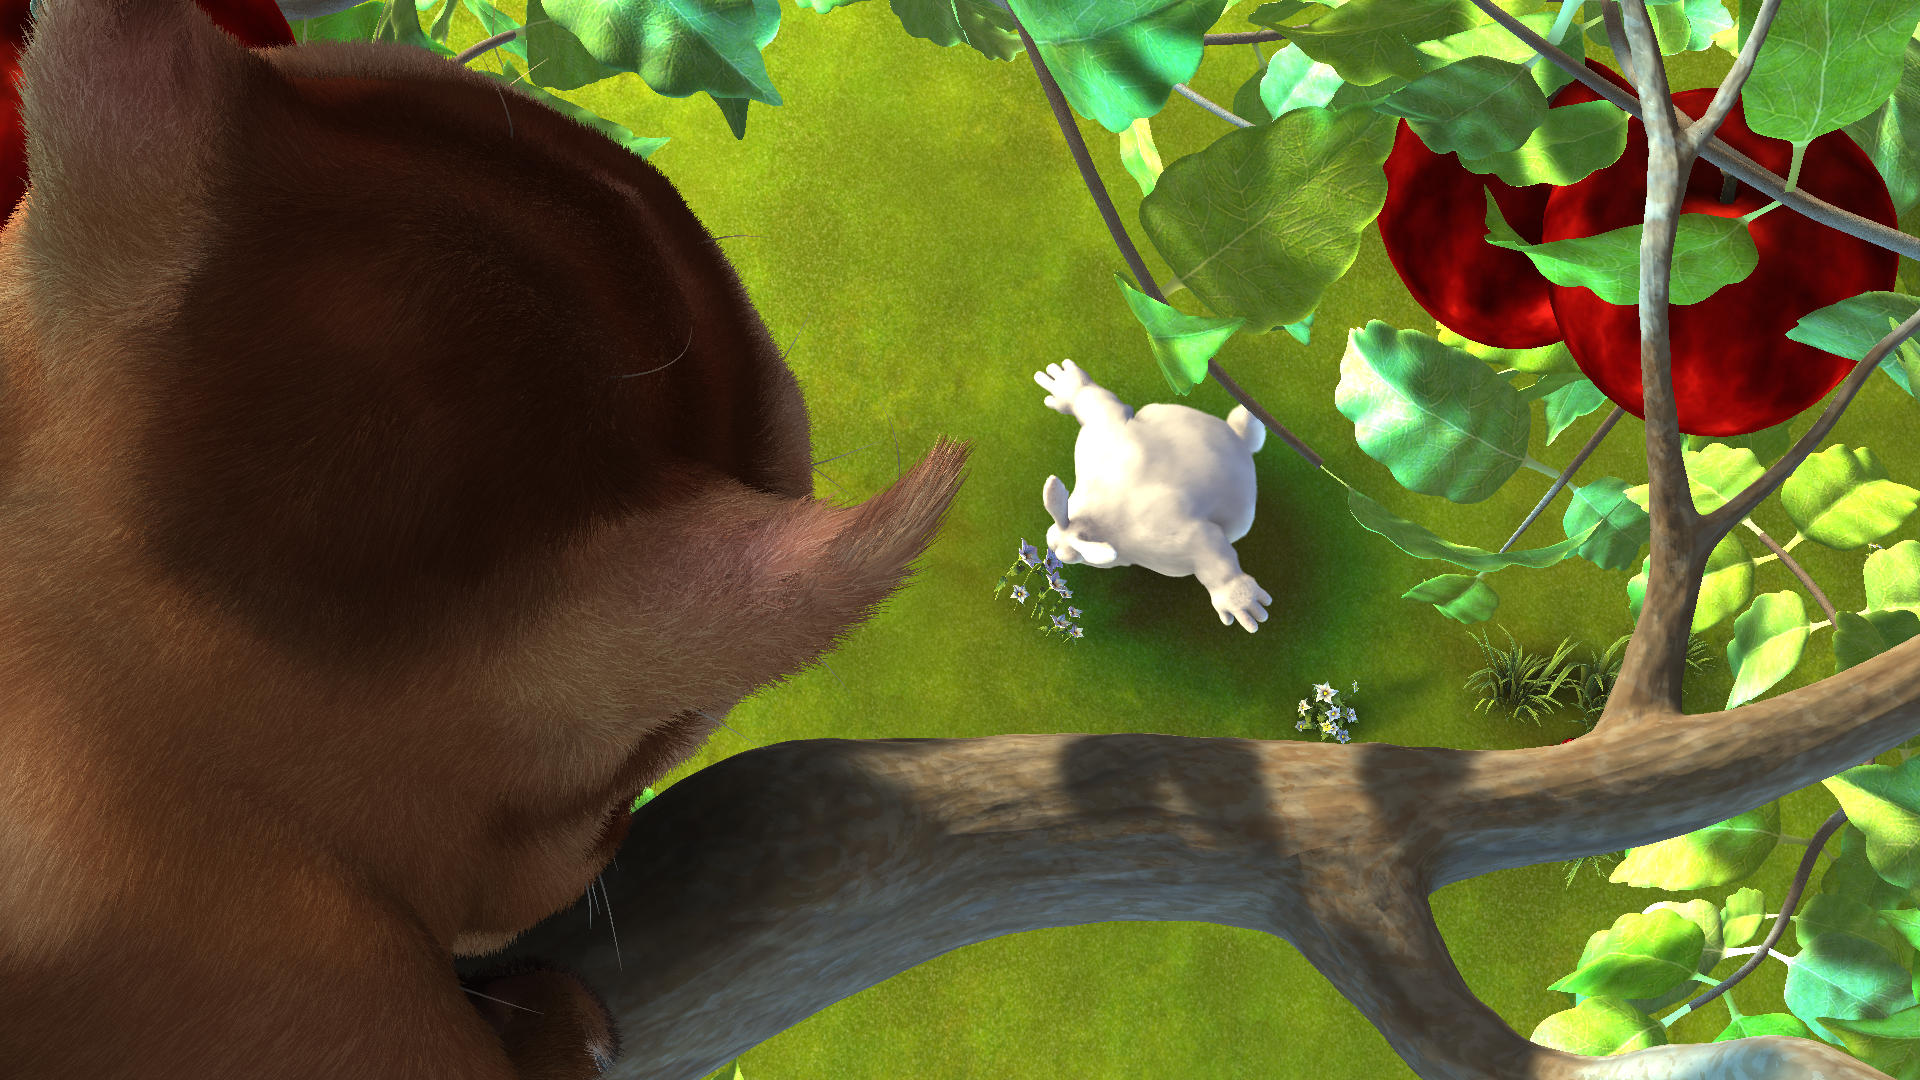
\includegraphics[width=0.47\textwidth]{src/images/svddd-03-left.png}} &
\subfloat[Right image]{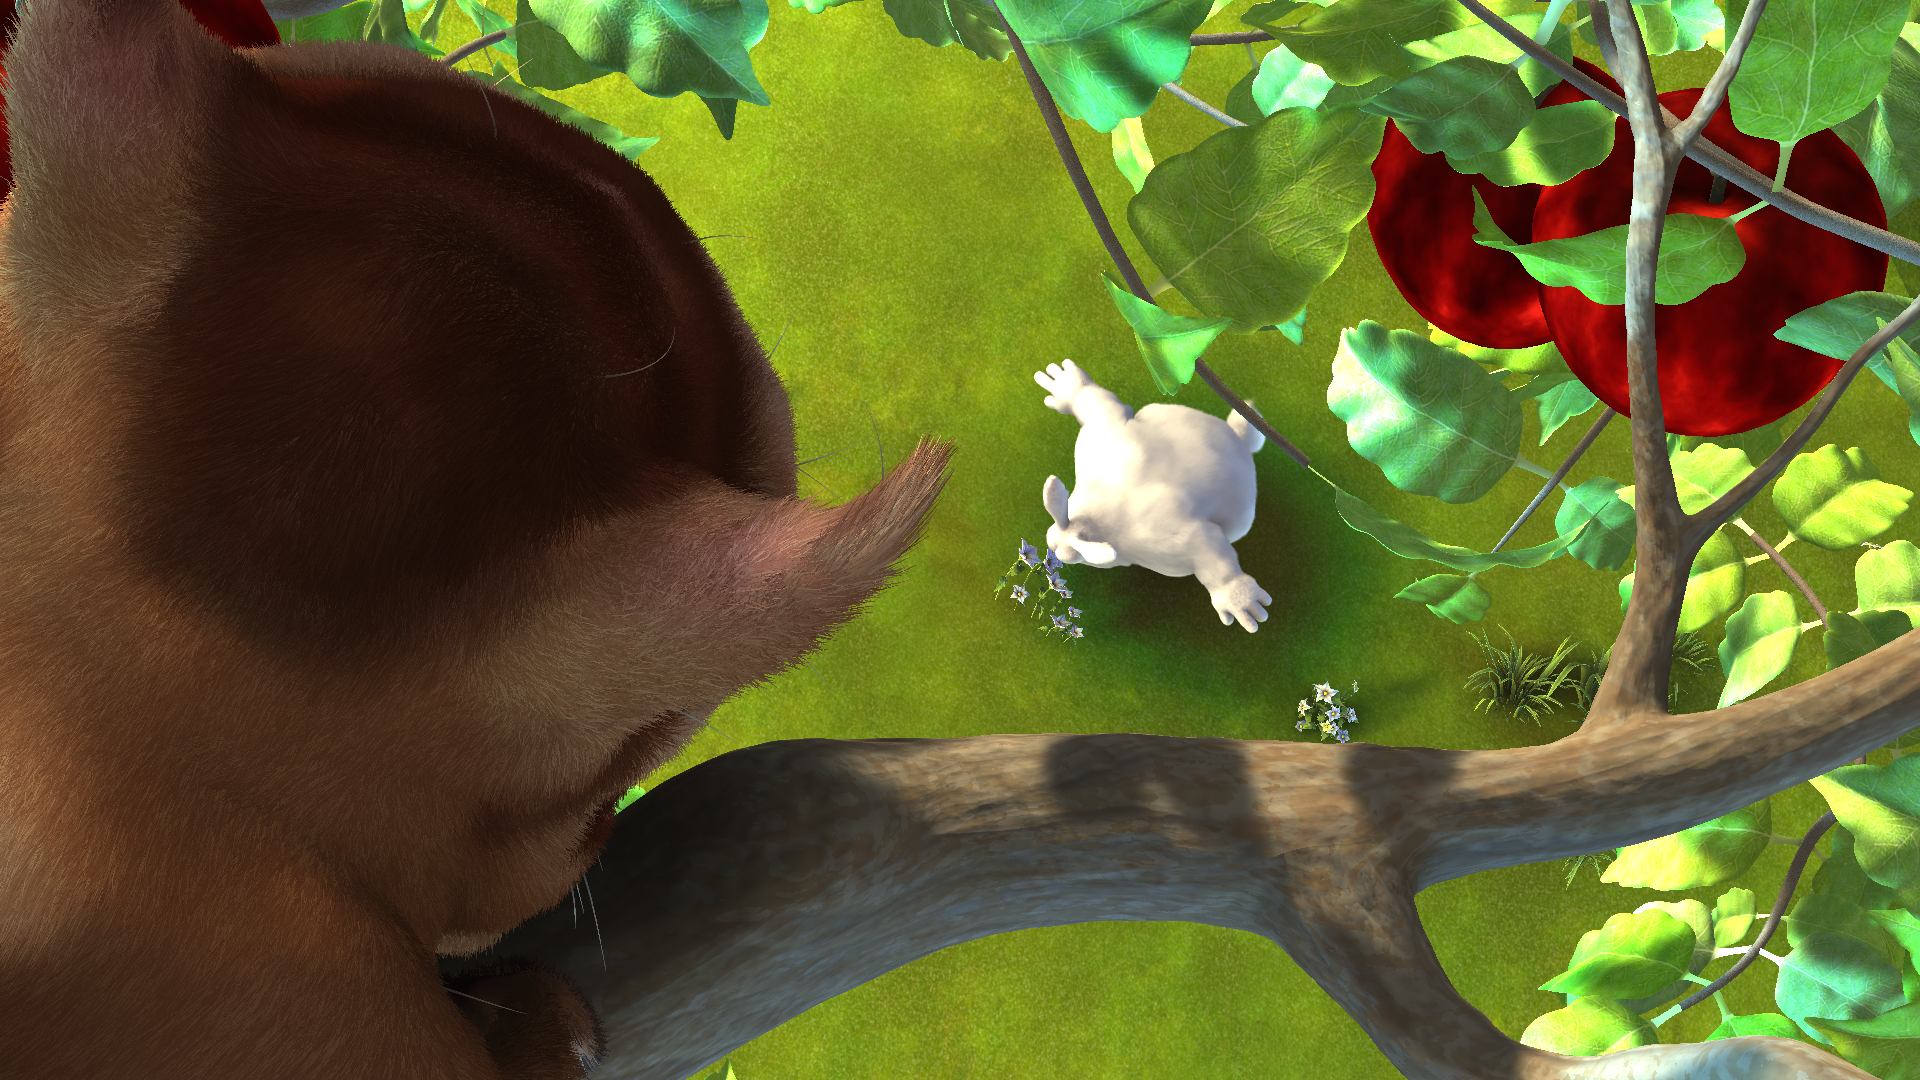
\includegraphics[width=0.47\textwidth]{src/images/svddd-03-right.png}} \\

\subfloat[Ground-truth disparity]{\includegraphics[width=0.47\textwidth]{src/images/svddd-03-heatmap-groundtruth.png}} &
\subfloat[SGBM output]{\includegraphics[width=0.47\textwidth]{src/images/svddd-03-heatmap-sgbm.png}} \\

\subfloat[MRF ICM output]{\includegraphics[width=0.47\textwidth]{src/images/svddd-03-heatmap-mrf.png}} &
\subfloat[ELAS output]{\includegraphics[width=0.47\textwidth]{src/images/svddd-03-heatmap-elas.png}} \\

\end{tabular}
\caption{Frame 01, scene 03 rabbit of the SVDDD dataset.}
\label{fig:svddd}
\end{figure}

\begin{figure}[h!]
  \centering
  \includegraphics[width=1.0\textwidth]{src/images/svddd-03-heatmap-outliers.png}
  \caption{Heatmap of outliers with threshold of 4.0 pixels in computed disparity map with OpenCV SGBM, frame 01, scene 03 rabbit, SVDDD dataset.}
  \label{fig:svddd-07}
\end{figure}

\subsubsection{Result matrix}

Insert overview matrix.

\subsection{Runtime}

Depict:

\begin{itemize}
  \item different performance of disparity algorithms,
  \item down-scaled performance,
  \item first down-scale, then run algorithms, then upscale, runtime,
  \item smoothing-over-time runtime.
\end{itemize}

\subsubsection{Result matrix}

\begin{landscape}
  \begin{table}[h!]
  \centering
  \begin{tabular}{cll|rrr}
    \hline
    \textbf{Rank} & \textbf{Method} & \textbf{Sequence} &  \textbf{Time} & \textbf{Time/MP} & \textbf{Quality index} \\ \hline \hline
    1 & StereoSGBM & SVDDD 02\_rabbit & 4.35\% & \cellcolor{green!60}5.43\% & 1.0 px \\
    2 & StereoBM & SVDDD 02\_rabbit & 4.35\% & 5.43\% & \cellcolor{red!60}1.1 px \\ \hline
  \end{tabular}
  \caption{Result matrix of runtime for videos}
  \label{tab:result-videos-runtime}
  \end{table}
\end{landscape}

\section{Discussion}

This is really important!




\chapter{Conclusion}
\label{chap:conclusion}

The work described in this thesis has been concerned with the comparison of disparity algorithms.
For this purpose, evaluation methods were introduced and integrated.
As stereoscopic datasets focusing on videos are rarely spread, the used ones for the evaluation were also introduced.
Additionally, a simple stereo matcher focusing on videos was implemented and thus described.
The following sections recap this in more detail and furthermore give a future outlook.

\section{Thesis summary}

\begin{itemize}
  \item What the thesis brought with each chapter.
  \item One small paragraph regarding one disparity algorithm.
  \item One small paragraph regarding dataset of the chair.
  \item What was implemented.
  \item What the main result of the evaluation.
\end{itemize}

%todo summarize a bit

The following modules were actually implemented:

\begin{itemize}
  \item Reader for the PFM file format.
  \item Python scripts for upcoming evaluation.
  \item Shell scripts for getting the docker containers and thus the work distributed among different instances\footnote{With instances virtual machines from DigitalOcean are meant.}.
  \item Evaluation processor for
\end{itemize}

%todo add recommendations for svddd dataset

\section{Future outlook}

A few thoughts on possible future work are outlined.
The thoughts are split in low- and high-level, from a technical perspective.
Low-level items are focused towards underlying methods of disparity algorithms, whereas high-level items focus on the bigger picture and tools which may help in developing stereo matcher.

\begin{itemize}
  \item Neuronal networks \citep{olshausen1996emergence}
  \item Other matching cost calculation methods \citep{hermann2010gradient}.
  \item Focus more on how humans experience depth? \citep{deangelis1995neuronal}
\end{itemize}

\begin{itemize}
  \item Real-time availability
  \item higher resolution
  \item What's on the market, like multi-view?
  \item Provide more real-world ground truth disparity maps \citep{kondermann2015stereo, Geiger2011IV}.
\end{itemize}


% End of main part
% ---------------------------------

% ---------------------------------
% Begin of appendix
\appendix
% Appendix chapters are optional. Use it if you have very long tables or additional figures that
% do not belong to the main text.
% \include{src/appendix}

% Remove this from the final document
% \chapter{Checklist}
\label{chap:appendix:checklist}
Use the following list to check if you have followed the hints from this document in your work.
Refer to \cref{chap:introduction} for more information on the items.

\tabulinesep=2.5mm
% tabu allows to use relative width specifier: Use X[<ratio>] to specify the width of a column. In
% this example, the table is divided into 20 parts that are spread over the three columns.
\begin{longtabu} to \textwidth {|X[1]|X[17]|X[2]|}
% Begin header on first page
\caption[Formatting checklist]{The checklist for correctly formatted and prettier documents.}
\label{tab:checklist}
\\
\hline
\endfirsthead
% End header on first page

% Begin header on consecutive pages
\caption[]{Table continued.}
\\
\hline
\endhead
% End header on consecutive pages

% Begin footer
\multicolumn{3}{c}{Table is continued on the next page.} \\
\endfoot
% End footer

% Begin footer on last page
\endlastfoot
% End footer on last page

% Begin content
1. & Check for incorrect/missing citations (\emph{[?]}) or references (\emph{??}). & \\
\hline
2. & Remove all \LaTeX{} errors and underfull/overfull boxes. & \\
\hline
3. & Make sure to use a consistent encoding for your \TeX{} files, especially for special characters (ä, ö, ü, ß, \dots). & \\
\hline
4. & Format your \textsc{Bib}\TeX{} document: Check if the information is correct and complete for each entry. Pay notice to warnings when running  the \texttt{bibtex} command.& \\
\hline
5. & Add access dates to online sources in your bibliography (see \texttt{library.bib}) or in footnotes. & \\
\hline
6. & Run a spell checker over your document (included with some \LaTeX{} editors). & \\
\hline
7. & Place figures or tables in the \TeX{} file at the end of the paragraph you are referring to them in the text (\texttt{\textbackslash{}ref}). & \\
\hline
8. & Use the correct format for quotation marks (\emph{``x''} or \emph{\glqq{}x\grqq{}}). & \\
\hline
9. & Use the correct format for separating paragraphs (one empty line). Manual line breaks (\texttt{\textbackslash{}\textbackslash}) should be avoided. & \\
\hline
10. & Use the correct form of dashes (-, --, ---). & \\
\hline
11. & Separate citations at the end of sentences/paragraphs with a small whitespace (\texttt{\~}). & \\
\hline
12. & Name sources of images/figures you did not create yourself in the description (\emph{Source: [X]}). & \\
\hline
13. & Use the short form of captions for List of Figures, Tables, etc. (\texttt{caption[<short>]\{<long>\}}). & \\
\hline
14. & If you print your work double-sided (recommended for bachelor and master thesis) remove the \texttt{oneside} option from the document class. & \\
\hline
15. & Make sure to use high-quality figures and images that are readable both in the digital and the printed version. & \\
\hline
16. & If you include the declaration of honor do not forget to sign it. & \\
\hline
% End content
\end{longtabu}

\backmatter

\bibliography{library}

\sloppy
\printglossary
\fussy

\declarationofhonorchap

Hiermit versichere ich, dass diese Arbeit von mir pers{\"o}nlich verfasst wurde und dass ich keinerlei fremde Hilfe in Anspruch genommen habe. Ebenso versichere ich, dass diese Arbeit oder Teile daraus weder von mir selbst noch von anderen als Leistungsnachweise andernorts eingereicht wurden. W{\"o}rtliche oder sinngem{\"a}ße {\"U}bernahmen aus anderen Schriften und Ver{\"o}ffentlichungen in gedruckter oder elektronischer Form sind gekennzeichnet. S{\"a}mtliche Sekund{\"a}rliteratur und sonstige Quellen sind nachgewiesen und in der Bibliographie aufgef{\"u}hrt. Das Gleiche gilt f{\"u}r graphische Darstellungen und Bilder sowie f{\"u}r alle Internet-Quellen.
Ich bin ferner damit einverstanden, dass meine Arbeit zum Zwecke eines Plagiatsabgleichs in elektronischer Form anonymisiert versendet und gespeichert werden kann.

\vspace{1cm}
\noindent
\insertcitydate{Mannheim}{3. Mai 2016}

\vspace{1.5cm}
\noindent
\insertauthor


% Consult your supervisor about the following declaration of assignment.
\begin{lang-de}
\chapter{Abtretungserklärung}
Hinsichtlich meiner Abschlussarbeit mit dem Titel \emph{\glqq{}\begin{lang-main}\inserttitle\end{lang-main}\grqq{}} räume ich der Universität Mannheim\fshyp{}Lehrstuhl für Praktische Informatik IV, Prof.\ Dr.\ Wolfgang Effelsberg, umfassende, ausschließliche unbefristete und unbeschränkte Nutzungsrechte an den entstandenen Arbeitsergebnissen ein.
Die Abtretung umfasst das Recht auf Nutzung der Arbeitsergebnisse in Forschung und Lehre, das Recht der Vervielfältigung, Verbreitung und Übersetzung sowie das Recht zur Bearbeitung und Änderung inklusive Nutzung der dabei entstehenden Ergebnisse, sowie das Recht zur Weiterübertragung auf Dritte.
\newline\newline\noindent Solange von mir erstellte Ergebnisse in der ursprünglichen oder in überarbeiteter Form verwendet werden, werde ich nach Maßgabe des Urheberrechts als Co\hyp{}Autor namentlich genannt.
Eine gewerbliche Nutzung ist von dieser Abtretung nicht mit umfasst.

\vspace{1cm}
\noindent
\insertcitydate{Mannheim}{Mai 2016}

\vspace{1.5cm}
\noindent
\insertauthor
\end{lang-de}

% End of appendix
% ---------------------------------

\end{document}
